% chapter macros
\DeclareRobustCommand{\ESF}{\mathrm{ESF}}
\DeclareRobustCommand{\PD}{\mathrm{PD}}
\DeclareRobustCommand{\GEM}{\mathrm{GEM}}
\DeclareRobustCommand{\Ex}{\mathbb{E}}
\DeclareRobustCommand{\Pr}{\mathbb{P}}
\DeclareRobustCommand{\Beta}{\mathrm{Beta}}
\DeclareRobustCommand{\Var}{\mathrm{Var}}
\chapter{Ascertainment and the Two Parameter Poisson Dirichlet Family}\label{ch:py}
\chaptermark{Ascertainment and Poisson Dirichlet}
\begin{chaptersummary}
Sampling a Poisson Dirichlet subdivision of the unit interval with a nonuniform density is a Rao
weighted distribution problem for Kingman's paintbox, and in the one parameter case it has an exact
answer: a $\Beta(1,\alpha)$ weight carries the Ewens sampling formula with parameter $\theta$ to the
one with parameter $\theta/\alpha$. We ask what survives in the two parameter family. Three things
happen. The reduction survives untouched, because its proof uses nothing about the law of the
subdivision. Exactness does not survive, and the obstruction is a rigidity theorem: the residual
allocation structure is preserved only by power weights, and among power weights the Ewens family
alone is preserved, so no sampling density that charges every interval carries the size biased sticks of $\PD(\sigma,\theta)$ with $\sigma>0$ to
the sticks of another member of the Ewens Pitman family. What replaces exactness is a first order law of the same
shape as the one parameter result, in which ascertainment multiplies the odds $(1-\sigma)/\sigma$ by
$\alpha$ and leaves the concentration $\theta$ untouched. Going further, the limiting
$\sigma$ diversity of the weighted problem is the unweighted one raised to a power, $S_* = CS^{\kappa}$
with $\kappa = \alpha\sigma_*/\sigma$ and $C$ in closed form, which follows from an identity between
the diversity and the stick envelope, $S = (M/\sigma)^{\sigma}$. Finally the coincidence theory of the
one parameter case collapses entirely: for $\sigma > 0$ the probability that no two intervals receive
the same number of points tends to zero under every weight with $\sigma_* > 0$. The abundance spectrum degenerates: every $A_j/n^{\sigma_*}$ converges to a deterministic multiple
of one random variable, so the shape of the spectrum is free of everything but $\sigma_*$. Two
consequences are practical. The singleton fraction $A_1/K_n$ estimates $\sigma_*$ with no
normalisation at all, and the bias from nonuniform sampling inverts exactly.
\end{chaptersummary}
\section{Introduction}
\label{py:sec:intro}

Warren Ewens asked what becomes of the Ewens sampling formula when the $n$ points dropped on a
Poisson Dirichlet subdivision of $(0,1)$ are sampled from a nonuniform density. In the
one parameter case the answer is unusually clean. Pushing the sample through the probability
integral transform absorbs the weighting into new paintbox frequencies, so the problem is a Rao
weighted distribution version of Kingman's paintbox. If the intervals are then laid down in
size biased rather than ranked order, a $\Beta(1,\alpha)$ density converts $\ESF(\theta)$ into
$\ESF(\theta/\alpha)$, exactly and at every sample size. In Sethuraman's stick breaking form the
same statement reads: ascertainment carries a Dirichlet process to a Dirichlet process, fixing the
base measure and the atoms and rescaling only the concentration.

The natural next question, and the one this chapter answers, is how much of that survives the
two parameter extension of Pitman and Yor. It is a fair question to ask sceptically. A result that
holds for a one parameter family and fails for its two parameter enlargement is often an accident of
the smaller family, and one wants to know which it is here.

\subsection{What we find}

The answer separates into three parts, and they behave differently.

\emph{The reduction is universal.} Lemma~\ref{py:lem:pit} uses nothing about the law of the
subdivision: not exchangeability of the atoms, not Poisson Dirichlet structure, not even that the
lengths are random. It is also free of the direction in which the intervals are laid, by
Lemma~\ref{py:lem:reflect}, so a density and a direction enter only through $G$. The density disappears into new paintbox frequencies and only the tail sums
remain. So the entire framework is available for $\PD(\sigma,\theta)$, for Ewens Pitman, and for
any other paintbox one cares to write down.

\emph{Exactness is exactly the Ewens case, and rigidly so.} Theorem~\ref{py:thm:rigid} says that the
residual allocation structure, independence of the successive stick factors, is preserved only by
power weights $G(r) = r^{\alpha}$, by a Cauchy equation that we derive through quantiles.
Theorem~\ref{py:thm:pitman} then says that among power weights the Ewens family alone is preserved.
Together these give the following statement: for $\sigma \in (0,1)$ no
sampling density that charges every interval, apart from the uniform, carries the size biased sticks of $\PD(\sigma,\theta)$ to the sticks of a member of the Ewens Pitman family. Whether a density could still produce an Ewens Pitman partition with the induced sticks out of size biased order is settled here only at particular parameter values (Section~\ref{py:sec:rigid}). The stability of the one parameter theory is therefore a coincidence between two
one parameter families rather than an instance of a general principle, and the two parameter case is
where one sees that.

\emph{The first order generalises, in the right coordinate.} Proposition~\ref{py:prop:pyimage} gives
\[
\frac{\log K_n}{\log n} \longrightarrow \sigma_* = \frac{\sigma}{\alpha(1-\sigma)+\sigma},
\qquad\text{equivalently}\qquad
\frac{1-\sigma}{\sigma} \longmapsto \alpha\,\frac{1-\sigma}{\sigma} .
\]
Ascertainment multiplies the odds of the discount parameter by $\alpha$, as it divides the Ewens
parameter by $\alpha$. The concentration $\theta$ does not appear.

Beyond the first order we can say more than we expected. The limiting $\sigma$ diversity satisfies
$S = (M/\sigma)^{\sigma}$, where $M$ is the stick envelope (Lemma~\ref{py:lem:MS}). The weighted
diversity is then $S_* = C S^{\kappa}$ almost surely (Proposition~\ref{py:prop:power}), with $C$ in
closed form and free of $\theta$ (Proposition~\ref{py:prop:constant}). So the weighting does not
produce a new random object: it reproduces the old one raised to a power. The abundance spectrum
follows suit, and degenerately: by Proposition~\ref{py:prop:joint} every $A_j/n^{\sigma_*}$ converges
to a deterministic multiple of the same $S_*$.

Section~\ref{py:sec:arbitrary} drops the Beta form altogether. For an arbitrary weight that charges every interval the exact theory
is gone, by Theorem~\ref{py:thm:rigid}. The asymptotic theory survives with the regular variation index
$\rho$ of $G$ in place of $\alpha$: the growth rates of $K_n$ fall into four regimes
(Theorem~\ref{py:thm:regimes}), the singleton fraction estimates $\sigma_*$ for every weight of positive index whose density is regularly varying at the far endpoint
(Corollary~\ref{py:cor:anyweight}), and $\rho$ itself can be read off recorded positions by Hill's
estimator (Corollary~\ref{py:cor:hill}).

Section~\ref{py:sec:coalescent} reads all of this genealogically. The coalescent derivation of the
one parameter formula cannot produce $\sigma > 0$: its type count is a sum of independent indicators
and the two parameter count is overdispersed (Proposition~\ref{py:prop:nocoal}). The two repairs in the
literature are the Chinese restaurant and multiple merger coalescents, and ascertainment biases the
index a geneticist would infer from either.

Section~\ref{py:sec:coincidence} records the one part of the one parameter theory that does not
survive at all. The probability that no two intervals receive the same number of points tends to
$e^{-\gamma\vartheta}/\Gamma(1+\vartheta)$ when $\sigma = 0$, where $\vartheta$ is the Ewens parameter of the sampled law ($\vartheta = \theta/\alpha$ under a $\Beta(1,\alpha)$ density), and to zero for every $\sigma > 0$
under every weight with $\sigma_* > 0$. Section~\ref{py:sec:estimation} draws the statistical consequence: an estimator of
$\sigma$ from a nonuniformly sampled population is biased in a way that inverts exactly, and we
give the correction.

\subsection{Why ``ascertainment''}
\label{py:sec:whyascertainment}

The word is inherited from human genetics, and it means what it says: a unit is \emph{ascertained}
when it comes to the investigator's attention, and the difficulty is that the probability of coming
to attention depends on the very quantity under study.

The canonical case is Fisher's. To estimate the segregation ratio for a recessive trait one collects
families and counts affected children, but families cannot be sampled at random, because a family
with no affected child never reaches a clinic. Families are found \emph{through} their affected
children. Under single ascertainment a family with $r$ affected children enters the sample with
probability proportional to $r$; if each affected child independently brings the family to attention
with probability $\pi$, the probability is $1-(1-\pi)^{r}$. Either way the sample overrepresents
families with many affected children and the naive ratio is biased upward.
\citet{py:fisher1934} derived the correction, formalising what Weinberg's proband method had attempted,
and ``ascertainment bias'' entered the vocabulary there.

\citet{py:rao1965} turned this into a general framework, in a paper titled, literally, ``On discrete
distributions arising out of methods of ascertainment''. Every such scheme has one structure: the
population has density $f$, a unit with value $x$ is ascertained with probability proportional to a
weight $w(x)$, and the sample follows the weighted density $w(x)f(x)/\Ex[w]$. Size biased sampling
is the case $w(x) = x$. \citet{py:patil1978} developed the framework for ecology and wildlife, which
is the lineage of the tired collector of Section~\ref{py:sec:example}.

In the present problem the weight is the sampling density itself. An interval of the paintbox is
ascertained, that is, receives at least one specimen, with probability governed by the mass the
density places on it, so the induced frequencies of Lemma~\ref{py:lem:pit} are the Rao weighted version
of the paintbox frequencies. This is why the confounding warning of Bayarri and DeGroot applies with
full force, and why it can be made exact here: the weight and the underlying law are learnable only
through a single combination, $\theta/\alpha$ in the one parameter case and
$\sigma_* = \sigma/\{\rho(1-\sigma)+\sigma\}$ in the two parameter one.

\subsection{Related work}

The weighted distribution formulation and its identifiability difficulty are set out in
Section~\ref{py:sec:whyascertainment}; the confounding is the theme of Bayarri and DeGroot's work on
the subject, and the present chapter is a case where it can be described exactly rather than warned
about. The paintbox is Kingman's \citep{py:kingman1978}, the one parameter sampling formula is Ewens's
\citep{py:ewens1972}, the stick breaking form we use throughout is Sethuraman's
\citep{py:sethuraman1994}, and the two parameter family, its partition probability function and
its $\sigma$ diversity are due to Pitman and Yor \citep{py:pitman1995,py:pitmanyor1997}, with
\citet{py:pitman2006} the standard account. The occupancy asymptotics we lean on, the
correspondence between the counting function of the frequencies and the growth of the number of
occupied cells, are Karlin's \citep{py:karlin1967}. What appears to be new here is the rigidity of Theorem~\ref{py:thm:rigid},
the exponent map of Proposition~\ref{py:prop:pyimage} and its odds form, and the diversity identities of
Section~\ref{py:sec:diversity}.

\subsection{Notation}

Write $\PD(\sigma,\theta)$ for the two parameter Poisson Dirichlet law, $0 \le \sigma < 1$ and
$\theta > -\sigma$, whose size biased stick fractions are independent with
\begin{equation}
B_k \sim \Beta(1-\sigma,\, \theta + k\sigma),
\qquad
W_k = B_k \prod_{i<k}(1-B_i),
\qquad
\widetilde R_k = \prod_{i \le k}(1-B_i).
\label{py:eq:pysticks}
\end{equation}
At $\sigma = 0$ this is $\GEM(\theta)$ and the induced partition of a uniform sample is
$\ESF(\theta)$. The subdivision of $(0,1)$ is laid down in some order, $n$ points are dropped with
density $f$ rather than uniformly, $F$ is its distribution function, and
\begin{equation}
G(r) = 1 - F(1-r),
\qquad
f_\alpha(x) = \alpha(1-x)^{\alpha-1} \iff G(r) = r^{\alpha}.
\label{py:eq:G}
\end{equation}
Here $\alpha > 1$ concentrates the sample near $x = 0$ and $\alpha < 1$ near $x = 1$. At $\sigma = 0$,
$\vartheta$ denotes the Ewens parameter of the sampled law: $\vartheta = \theta$ under uniform
sampling and $\vartheta = \theta/\alpha$ under $f_\alpha$. We take the
layout to run from the left throughout, which by Lemma~\ref{py:lem:reflect} costs no generality. Write $A_j$
for the number of intervals hit exactly $j$ times, $K_n = \sum_j A_j$ for the number of intervals
hit at all, and $N(x) = \#\{k : p_k > x\}$ for the counting function of the induced frequencies.
Rising factorials are written $(x)_m = x(x+1)\cdots(x+m-1)$, with $(x)_0 = 1$, and the odds of the
discount parameter, $(1-\sigma)/\sigma$, are written $\beta$ inside proofs and $\omega$ when they
are viewed as a coordinate on the parameter space.

\subsection{Small samples by hand}
\label{py:sec:small}

Before any asymptotics it helps to have the exact law of a small sample in front of us, because
several statements below (the exact one parameter theorem, its failure at $\sigma > 0$) are
statements about these finite dimensional laws. Under uniform sampling the probability that the
partition of $\{1,\dots,n\}$ induced by a $\PD(\sigma,\theta)$ paintbox equals a particular set
partition with $k$ blocks of sizes $n_1,\dots,n_k$ is Pitman's exchangeable partition probability
function \citep{py:pitman1995},
\begin{equation}
p_{\sigma,\theta}(n_1,\dots,n_k) \;=\;
\frac{\prod_{i=1}^{k-1}(\theta+i\sigma)}{(\theta+1)_{n-1}}\;\prod_{j=1}^{k}(1-\sigma)_{n_j-1} .
\label{py:eq:eppf}
\end{equation}
At $\sigma = 0$ this is the Ewens sampling formula written for a single set partition,
$\theta^{k-1}\prod_j (n_j-1)!/(\theta+1)_{n-1}$. The probability of a partition \emph{type}, a
multiset of block sizes, is \eqref{py:eq:eppf} multiplied by the number of set partitions of that
type: for $n = 4$ these multiplicities are $1, 4, 3, 6, 1$ for the types $4$, $3{+}1$, $2{+}2$,
$2{+}1{+}1$ and $1{+}1{+}1{+}1$, fifteen set partitions in all.

\begin{example}[Pitman's formula at $n = 3$ and $n = 4$]
\label{py:ex:eppf}
Take $(\sigma,\theta) = (\tfrac12, 1)$ and the set partition $\{1,2\}\{3\}\{4\}$. Here $k = 3$, the
numerator is $(\theta+\sigma)(\theta+2\sigma) = \tfrac32\cdot 2 = 3$, the denominator is
$(2)_3 = 2\cdot3\cdot4 = 24$, and the block factors are $(\tfrac12)_1 = \tfrac12$ for the pair and
$1$ for each singleton. So $p = 3/48 = 1/16$, and the type $2{+}1{+}1$ has probability
$6/16 = 3/8$. Table~\ref{py:tab:eppf} lists every type for $n = 3$ and $n = 4$ under five parameter
pairs; each column sums to one, which is a useful check on \eqref{py:eq:eppf}.

Three things are visible in the table. First, at $n = 2$ the formula gives the chance that two
sampled genes are of the same allele, the homozygosity
\[
\Pr(\text{two draws in one block}) \;=\; \frac{1-\sigma}{1+\theta},
\]
which is $1/(1+\theta)$ in the Ewens case. One number cannot separate $\sigma$ from $\theta$; the
pairs $(0,1)$ and $(\tfrac12,0)$ both give $\tfrac12$. Second, the two pairs are separated at
$n = 3$: the probability that all three draws agree is $(1-\sigma)(2-\sigma)/\{(1+\theta)(2+\theta)\}$,
which is $\tfrac13$ for $(0,1)$ and $\tfrac38$ for $(\tfrac12,0)$. Third, at a fixed homozygosity a positive $\sigma$ moves
mass to both extremes at once: compared with $\ESF(1)$, the law $\PD(\tfrac12,0)$ puts more
probability on a single block of four ($5/16$ against $1/4$) and more on four distinct blocks
($1/8$ against $1/24$), less on the shapes $3{+}1$ and $2{+}2$, and the same on $2{+}1{+}1$. A few very common types together with
many rare ones is the small sample face of the heavy tail.
\end{example}

\begin{table}[t]
\centering
\caption{Exact probabilities of each partition type at $n = 3$ and $n = 4$ under
\eqref{py:eq:eppf}. Each column, headed by a pair $(\sigma,\theta)$, gives the probability of the whole type,
including its multiplicity.}
\label{py:tab:eppf}
\small
\begin{adjustbox}{max width=\textwidth}
\begin{tabular}{llrrrrr}
\toprule
$n$ & type & $(0,1)$ & $(0,2)$ & $(\tfrac12,0)$ & $(\tfrac12,1)$ & $(\tfrac14,2)$\\
\midrule
$3$ & $3$     & $1/3$ & $1/6$ & $3/8$ & $1/8$ & $7/64$\\
    & $2{+}1$ & $1/2$ & $1/2$ & $3/8$ & $3/8$ & $27/64$\\
    & $1{+}1{+}1$ & $1/6$ & $1/3$ & $1/4$ & $1/2$ & $15/32$\\
\midrule
$4$ & $4$     & $1/4$ & $1/10$ & $5/16$ & $5/64$ & $77/1280$\\
    & $3{+}1$ & $1/3$ & $4/15$ & $1/4$ & $3/16$ & $63/320$\\
    & $2{+}2$ & $1/8$ & $1/10$ & $1/16$ & $3/64$ & $81/1280$\\
    & $2{+}1{+}1$ & $1/4$ & $2/5$ & $1/4$ & $3/8$ & $27/64$\\
    & $1{+}1{+}1{+}1$ & $1/24$ & $2/15$ & $1/8$ & $5/16$ & $33/128$\\
\bottomrule
\end{tabular}
\end{adjustbox}
\end{table}

\subsection{An occupancy lemma}
\label{py:sec:karlin}

Most asymptotic statements in this chapter pass from the induced frequencies to the counts through
one correspondence, due to \citet{py:karlin1967}, and we state it once so that later proofs can cite
it rather than gesture at it. Throughout, the frequencies are held fixed (we condition on the
paintbox) and $L$ denotes a slowly varying function.

\begin{lemma}[Karlin's occupancy correspondence]
\label{py:lem:karlin}
Let $(p_k)$ be a fixed probability sequence with counting function $N(x) = \#\{k : p_k > x\}$,
and suppose $N(x) = x^{-\gamma}L(1/x)$ as $x \downarrow 0$ for some $\gamma \in (0,1)$. Then, for
an i.i.d.\ sample of size $n$ from $(p_k)$,
\[
K_n \sim \Gamma(1-\gamma)\,n^{\gamma}L(n)
\quad\text{and}\quad
A_j \sim \frac{\gamma\,\Gamma(j-\gamma)}{j!}\,n^{\gamma}L(n)
\]
almost surely, the second for each fixed $j \ge 1$.
If instead $N(x) \sim c\log(1/x)$, then $K_n \sim c\log n$ almost surely. In the boundary case $\gamma = 1$, $N(x) = x^{-1}L(1/x)$, the function $L_1(y) = \int_y^\infty L(u)u^{-1}du$ is finite and slowly varying with $L_1(y)/L(y) \to \infty$, and
\[
K_n \;\sim\; nL_1(n) \;=\; \sum_k \min(np_k,\,1)
\]
almost surely; so $K_n/n \to 0$, but more slowly than any negative power of $n$.
\end{lemma}

\begin{proof}[Proof sketch]
Replace the fixed sample size by a Poisson number of draws with mean $t$, so that the cells are
filled independently and cell $k$ is occupied with probability $1-e^{-tp_k}$. Writing the sum over
cells as a Stieltjes integral against $-dN$ and integrating by parts,
\[
\Ex[K(t)] \;=\; \sum_k\big(1-e^{-tp_k}\big)
\;=\; \int_0^\infty t e^{-tx}N(x)\,dx
\;=\; \int_0^\infty e^{-u}N(u/t)\,du .
\]
The boundary terms vanish because $N(x) = 0$ for $x \ge 1$ and $xN(x) \to 0$ as $x \downarrow 0$, the
latter since $xN(x) \le x N(\varepsilon) + \sum_{k:\,p_k \le \varepsilon}p_k$ for every
$\varepsilon > 0$. Now $N(u/t) = t^{\gamma}u^{-\gamma}L(t/u)$, and $L(t/u)/L(t) \to 1$ for each
$u$; Potter's bounds for slowly varying functions dominate the ratio by a multiple of
$u^{-\delta}+u^{\delta}$ for small $\delta > 0$, so dominated convergence gives
$\Ex[K(t)] \sim t^{\gamma}L(t)\int_0^\infty u^{-\gamma}e^{-u}du = \Gamma(1-\gamma)t^{\gamma}L(t)$.
The same calculation with $(tx)^{j}e^{-tx}/j!$ in place of $1-e^{-tx}$ gives the mean of $A_j$,
after one integration by parts:
$\Ex[A_j(t)] = \int_0^\infty \pi_j'(u)N(u/t)\,du$ with $\pi_j(u) = u^je^{-u}/j!$, and
$\int_0^\infty \pi_j'(u)\,u^{-\gamma}du = \gamma\int_0^\infty \pi_j(u)u^{-\gamma-1}du
= \gamma\Gamma(j-\gamma)/j!$. In the Poissonised scheme $K(t)$ is a sum of independent indicators,
so $\Var K(t) \le \Ex K(t)$; Chebyshev's inequality along $t_m = (1+\eta)^{m}$ and the
Borel and Cantelli lemma give $K(t_m)/\Ex K(t_m) \to 1$ almost surely, and monotonicity of $K$ in
$t$ fills the gaps up to a factor $(1+\eta)^{\gamma}$, which is released as $\eta \downarrow 0$.
Finally a Poisson variable with mean $t$ lies in $[t-t^{2/3},\,t+t^{2/3}]$ eventually, and $K_n$ is
monotone in $n$, so the statement transfers to fixed $n$. The counts $A_j$ are not monotone in
$n$, but each is a difference of the monotone quantities $\#\{k : \text{count}_k \ge j\}$, which
are handled the same way. The logarithmic case is identical with $c\log t$ in place of
$t^{\gamma}L(t)$.

At $\gamma = 1$ the constant $\Gamma(1-\gamma)$ is infinite and the mean needs a different treatment. The substitution $y = 1/x$ turns $\int_0^1 N(x)\,dx = \sum_k p_k = 1$ into $\int_1^\infty L(y)y^{-1}dy = 1$, so $L_1$ is finite, and $\int_0^{1/t}N(x)\,dx = \sum_k\min(p_k,1/t)$ is $L_1(t)$. For $\lambda > 1$, $L_1(y)-L_1(\lambda y) = \int_y^{\lambda y}L(u)u^{-1}du \sim L(y)\log\lambda$, so $\liminf L_1(y)/L(y) \ge \log\lambda$ for every $\lambda$; hence $L_1/L \to \infty$ and $L_1(\lambda y)/L_1(y) \to 1$. Now split $\Ex[K(t)] = t\int_0^\infty e^{-u}u^{-1}L(t/u)\,du$ at $u = 1$. The part $u > 1$ is $O(L(t))$ by Potter's bounds, which is $o(L_1(t))$. The part $u \le 1$ is $\int_t^\infty e^{-t/y}L(y)y^{-1}dy$, which lies between $e^{-1/\lambda}L_1(\lambda t)$ and $L_1(t)$; since $L_1(\lambda t) \sim L_1(t)$ and $\lambda$ is arbitrary, it is $L_1(t)(1+o(1))$. So $\Ex[K(t)] \sim tL_1(t)$, which is regularly varying with index one, and the almost sure statement and the passage to fixed $n$ go through as before.
\end{proof}

Two features of the lemma recur below. The constant $\Gamma(1-\gamma)$ is the only place the
sampling enters: everything else is a property of the frequencies. And the profile
$\gamma\Gamma(j-\gamma)/j!$ of the counts depends on $\gamma$ alone, which is the source of every
estimator of $\sigma$ in Section~\ref{py:sec:estimation}.

\section{The reduction, and why it is universal}
\label{py:sec:reduction}

\begin{lemma}[Reduction]
\label{py:lem:pit}
Let the intervals be laid down in any order, with tail sums $R_k$, and let $X_1,\dots,X_n$ be
i.i.d.\ with density $f$. Then the induced partition of $\{1,\dots,n\}$ is a Kingman paintbox with
frequencies
\[
p_k \;=\; \Pr(X \in V_k) \;=\; G(R_{k-1}) - G(R_k),
\qquad \sum_k p_k = 1 .
\]
\end{lemma}

\begin{proof}
The $k$th interval is $(1-R_{k-1},\,1-R_k]$, so $\Pr(X \in V_k) = F(1-R_k) - F(1-R_{k-1})$, which is
$G(R_{k-1})-G(R_k)$ by \eqref{py:eq:G}. The sum telescopes to $G(1)-\lim_k G(R_k) = 1$ since
$R_k \downarrow 0$ and $G$ is continuous at the origin. The points remain i.i.d., so the induced
partition is exchangeable and is the paintbox with those frequencies.
\end{proof}

Two structural facts follow and hold for every paintbox. Under uniform sampling $G(r) = r$ gives
$p_k = V_k$ for every arrangement, so the order the atoms are laid down in is irrelevant, which is
why the classical theory never mentions it. Under any other weight the order matters, because
$p_k$ depends on where the $k$th interval sits and not only on how long it is. And the induced
frequencies are again a paintbox, so we have not left Kingman's framework but moved inside it, from
one paintbox to another. Everything that follows is a question about which laws of $(R_k)$ leave
the new frequencies tractable.

Figure~\ref{py:fig:construction} shows the objects. The lower panel is a ranked $\PD(0.5,1)$
subdivision; the upper panel is the sampling density for three values of $\alpha$. A collector
using $\alpha = 3$ takes almost half of the sample from the first fifth of the interval, which under a
ranked layout is where the large atoms are, so a few atoms absorb almost all of the mass. A
collector using $\alpha = 0.5$ does the reverse and reaches deep into the dust.

\begin{figure}[t]
\centering
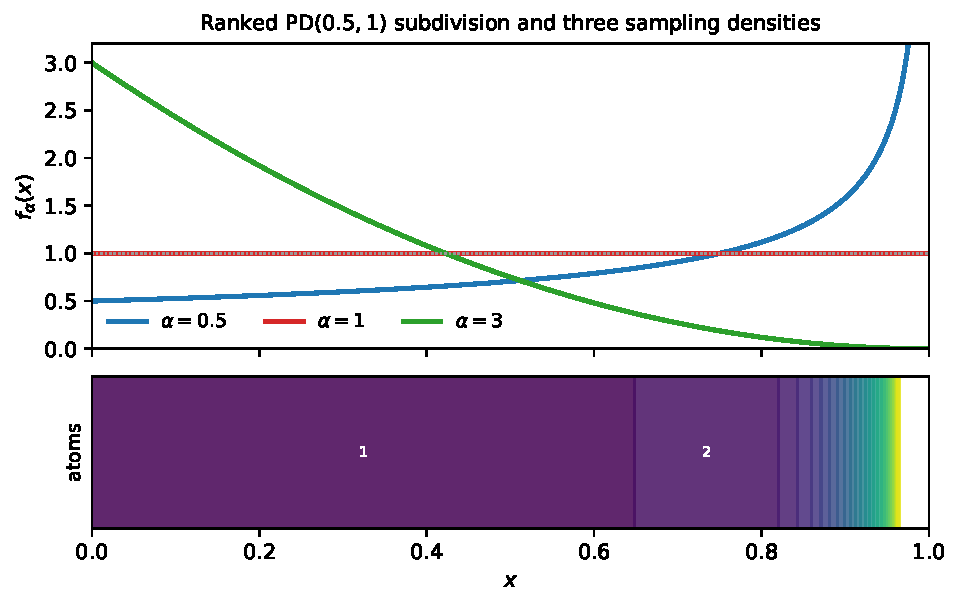
\includegraphics[width=0.86\textwidth]{figures/py_fig-construction.pdf}
\caption{The construction. Below, a ranked $\PD(0.5,1)$ subdivision of $(0,1)$, the first
twenty five atoms shaded and the largest few labelled. Above, the sampling densities $f_\alpha$ for
$\alpha = 0.5$, $1$ and $3$. Uniform sampling is the dotted line; every other density makes the
position of an atom, and not merely its length, matter.}
\label{py:fig:construction}
\end{figure}

\subsection{The direction of the layout, and a reflection}
\label{py:sec:direction}

Lemma~\ref{py:lem:pit} was stated for intervals laid down from the left, so that the $k$th interval is
$(1-R_{k-1},\,1-R_k]$ and the weight enters through $G(r) = 1-F(1-r)$. Nothing forces that choice,
and the alternative is not a new case.

\begin{lemma}[Reflection]
\label{py:lem:reflect}
Fix a subdivision with tail sums $(R_k)$. Lay the intervals from the left and sample with density
$f$; or lay them from the right, so that the $k$th interval is $(R_k,\,R_{k-1}]$, and sample with
the reflected density $\check f(x) = f(1-x)$. The induced frequencies coincide, both being
$G(R_{k-1})-G(R_k)$ with $G(r) = 1-F(1-r)$.
\end{lemma}

\begin{proof}
The reflected distribution function is $\check F(x) = 1-F(1-x) = G(x)$. Laid from the right, the
$k$th frequency is $\check F(R_{k-1})-\check F(R_k)$, which is $G(R_{k-1})-G(R_k)$.
\end{proof}

So a density and a direction are not two pieces of data but one. Everything that follows is a
statement about $G$ alone, and a table of arrangements against densities collapses to a table of
values of $G$. Table~\ref{py:tab:onepar} records the collapse at $\sigma = 0$, where the exact theory
lives.

\begin{table}[t]
\centering
\caption{The one parameter cases, reduced to $G$. The size biased layout is a residual allocation
model in either direction; the ranked layout is not. The image is $\ESF$ when $G$ is a power and
the layout is size biased; rows four and five are not $\ESF$ at the values checked in the text.}
\label{py:tab:onepar}
\small
\begin{adjustbox}{max width=\textwidth}
\begin{tabular}{llll}
\toprule
layout & density & $G(r)$ & image \\
\midrule
size biased, from the left & $1$ & $r$ & $\ESF(\theta)$ \\
size biased, from the left & $\alpha(1-x)^{\alpha-1}$ & $r^{\alpha}$ & $\ESF(\theta/\alpha)$ \\
size biased, from the right & $\alpha x^{\alpha-1}$ & $r^{\alpha}$ & $\ESF(\theta/\alpha)$ \\
size biased, from the left & $\alpha x^{\alpha-1}$ & $1-(1-r)^{\alpha}$ & not $\ESF$; $K_n \sim \theta\log n$ \\
ranked, either direction & $\alpha(1-x)^{\alpha-1}$ & $r^{\alpha}$ &
  not $\ESF$; $K_n \sim (\theta/\alpha)\log n$ \\
\bottomrule
\end{tabular}
\end{adjustbox}
\end{table}

Rows two and three are one statement by Lemma~\ref{py:lem:reflect}. Taking $\alpha = \theta$ in either
gives $\ESF(1)$: the weight $\theta(1-x)^{\theta-1}$ undoes the stick breaking exactly, since its
distribution function is the one that carries each $\Beta(\theta,1)$ residual factor to a uniform.
Rows four and five are the two ways exactness can fail, and they fail for different reasons. In row
four $G$ is not multiplicative, which is the failure Theorem~\ref{py:thm:rigid} shows to be generic. In
row five $G$ is multiplicative but the layout is not a residual allocation model, so
Theorem~\ref{py:thm:rigid} does not apply in the first place. The two conditions, $G(r) = r^{\alpha}$
and a size biased layout, are independent, and exactness needs both. The check is at $n = 2$: if
$K_n \sim c\log n$ the only candidate law is $\ESF(c)$, under which two points share an interval
with probability $1/(1+c)$, and at $\theta = 1$, $\alpha = 2$ row four gives $0.445$ against $1/2$
and row five gives $0.728$ against $2/3$.

The last column of Table~\ref{py:tab:onepar} is asymptotic in its last two rows, and those are the
content of the next two statements.

\begin{proposition}[The index is the contact order at the far endpoint]
\label{py:prop:contact}
Let the intervals be laid from the left and let $f$ be continuous on $(0,1)$ with
$f(x) \sim a(1-x)^{\alpha-1}$ as $x \uparrow 1$, for some $a > 0$ and $\alpha > 0$. Then
\[
G(r) = \int_0^r f(1-u)\,du \;\sim\; \frac{a}{\alpha}\,r^{\alpha},
\qquad r \downarrow 0,
\]
so the density $G'(r) = f(1-r) \sim a\,r^{\alpha-1}$ is regularly varying at the origin with index
$\alpha-1$, $G$ is regularly varying with index $\rho = \alpha$, and
Proposition~\ref{py:prop:index} below applies with that $\rho$. Since $G'(r)/r^{\alpha-1} \to \alpha\,(a/\alpha)$,
the density condition of Section~\ref{py:sec:survives} holds with $c = a/\alpha$, and in the size biased layout
$S_* = (a/\alpha)^{\sigma_*}C\,S^{\kappa}$ with $C$ the constant of \eqref{py:eq:C}.
\end{proposition}

Only the behaviour of the sampling density at the endpoint the layout runs towards matters, and it
matters through one number. Two consequences answer the cases that looked intractable.

If $f$ has a positive finite limit $a$ at the far endpoint, then $\alpha = 1$ and $\rho = 1$, so
$\sigma_* = \sigma$ and $\kappa = 1$. The weight does not move the exponent at all, in either
family; its whole effect is the constant $a^{\sigma}$ multiplying the diversity. Row four of
Table~\ref{py:tab:onepar} is this case with $a = \alpha$: sampling a forward size biased layout with
$\alpha x^{\alpha-1}$ gives no exact law, but $\sigma_* = \sigma$ and $S_* = \alpha^{\sigma}S$
almost surely, and at $\sigma = 0$ it gives $K_n \sim \theta\log n$ with the concentration
untouched. The absence of a clean exact form is not the absence of an effect to report; the effect
is a scale factor and nothing more.

If $f$ vanishes at the far endpoint, $\alpha > 1$, the collector is fading and the exponent falls;
if $f$ blows up there, $\alpha < 1$, he is persistent and it rises. This is the reading of $\alpha$
given after Proposition~\ref{py:prop:pyimage}, now attached to the density rather than to $G$.

\begin{proposition}[The ranked layout at $\sigma = 0$]
\label{py:prop:ranked0}
Lay the $\PD(\theta)$ atoms in decreasing order and sample with $f_\alpha$. Then
$K_n/\log n \to \theta/\alpha$ almost surely, although at the values $\alpha \neq 1$ computed below
and in the discussion of Table~\ref{py:tab:onepar} the induced partition is not $\ESF(\theta/\alpha)$.
\end{proposition}

\begin{proof}
The ranked $\PD(\theta)$ atoms satisfy $-k^{-1}\log V_{(k)} \to 1/\theta$ almost surely, so
$R_k = \sum_{i>k}V_{(i)} = e^{-k(1+o(1))/\theta}$ and, by Lemma~\ref{py:lem:pit},
$R_k^{\alpha} = e^{-\alpha k(1+o(1))/\theta}$. Differencing, the induced frequencies have counting
function $N(x) = (\theta/\alpha)\log(1/x)\,(1+o(1))$, and Karlin's occupancy correspondence in the
logarithmic case converts this to $K_n = (\theta/\alpha)\log n\,(1+o(1))$. That the partition is not
$\ESF$ does not follow from Theorem~\ref{py:thm:rigid}, which concerns the size biased layout (see the
discussion of Table~\ref{py:tab:onepar}), but is a computation: for $\theta = \alpha = 2$ the ranked layout puts
two points in the same interval with probability about $0.56$, against $1/2$ for $\ESF(1)$, and
Table~\ref{py:tab:onepar_sim} shows the difference at $n = 4$.
\end{proof}

\begin{remark}
\label{py:rem:samestatement}
Propositions~\ref{py:prop:ranked0} and \ref{py:prop:layout} are the same statement in the two families. In
both, the arrangement of the atoms decides exactness and is invisible to the leading order, and in
both the constant is known in closed form only in the size biased layout. What changes across the
families is not the role of the layout but what survives it: at $\sigma = 0$ the leading order
retains the whole parameter map $\theta \mapsto \theta/\alpha$, while at $\sigma > 0$ it retains the
exponent map \eqref{py:eq:odds} and loses the law.
\end{remark}

\section{Rigidity: no weight preserves the two parameter family}
\label{py:sec:rigid}

In the one parameter case the exact theory rests on a single line. In size biased order
$G(r) = r^{\alpha}$ gives induced residual
$\widetilde R_k^{\,\alpha} = \prod_{i\le k}(1-B_i)^{\alpha}$, and for $\sigma = 0$ the factors
satisfy
\begin{equation}
1 - B_i \sim \Beta(\theta,1) \overset{d}{=} U^{1/\theta}
\quad\Longrightarrow\quad
(1-B_i)^{\alpha} \overset{d}{=} U^{\alpha/\theta} \sim \Beta(\theta/\alpha, 1),
\label{py:eq:oneline}
\end{equation}
so the induced subdivision is $\GEM(\theta/\alpha)$ and the catch is exactly $\ESF(\theta/\alpha)$
at every $n$. The middle equality in \eqref{py:eq:oneline} is the whole calculation: if
$\Pr(1-B \le u) = u^{\theta}$ then $\Pr\{(1-B)^{\alpha} \le v\} = \Pr(1-B \le v^{1/\alpha}) =
v^{\theta/\alpha}$, which is the distribution function of $\Beta(\theta/\alpha,1)$. Independence
of the factors is untouched because each is transformed separately.

\begin{example}[The one parameter theorem by simulation]
\label{py:ex:onepar}
Take $\theta = 2$ and $\alpha = 2$, so the theorem predicts that a sample drawn with density
$f_2(x) = 2(1-x)$ from a size biased $\GEM(2)$ subdivision has exactly the law $\ESF(1)$, although
under uniform sampling the same subdivision gives $\ESF(2)$. The two laws are far apart at
$n = 4$: by Table~\ref{py:tab:eppf}, $\ESF(1)$ puts probability $1/4$ on a single block and
$1/24$ on four singletons, while $\ESF(2)$ puts $1/10$ and $2/15$.

To check this we simulated $10^{6}$ weighted paintboxes. Each replicate draws eighty sticks
$B_k \sim \Beta(1,2)$, lays them from the left, and drops four points with $1-X = U^{1/2}$, so that
$\Pr(1-X \le r) = r^{2} = G(r)$. The omitted mass after eighty sticks has mean $(2/3)^{80}$, below
$10^{-14}$, so the truncation is invisible. Table~\ref{py:tab:onepar_sim} gives the frequencies of
the five types. In the size biased layout every one agrees with $\ESF(1)$ to within two
standard errors, and none is anywhere near $\ESF(2)$. Sorting the same sticks into decreasing order
before laying them down, and changing nothing else, gives the last column, which is neither law:
the ranked layout puts the largest atoms where the fading collector works hardest, so a single block
becomes more likely ($0.315$) and four singletons less likely ($0.023$) than under $\ESF(1)$. That
column is Proposition~\ref{py:prop:ranked0} at work: the same $G$, the same leading order
$(\theta/\alpha)\log n$, and no exact law.

An exact check is also available. The moment recursion of Example~\ref{py:ex:n4} below, run with
$\sigma = 0$, returns the probabilities $1/4$, $1/12$, $1/24$, $1/24$, $1/24$ for the five set
partition shapes to six decimal places, which are the $\ESF(1)$ values of \eqref{py:eq:eppf}.
\end{example}

\begin{table}[t]
\centering
\caption{Partition types of $n = 4$ points sampled with density $2(1-x)$ from a $\GEM(2)$
subdivision, over $10^{6}$ replicates; standard errors are at most $0.0005$. The theorem predicts
$\ESF(1)$ in the size biased layout. The ranked layout uses the same sticks sorted.}
\label{py:tab:onepar_sim}
\small
\begin{adjustbox}{max width=\textwidth}
\begin{tabular}{lrrrr}
\toprule
type & size biased, simulated & $\ESF(1)$ & $\ESF(2)$ & ranked, simulated\\
\midrule
$4$             & $0.2499$ & $0.2500$ & $0.1000$ & $0.3146$\\
$3{+}1$         & $0.3337$ & $0.3333$ & $0.2667$ & $0.3575$\\
$2{+}2$         & $0.1253$ & $0.1250$ & $0.1000$ & $0.1134$\\
$2{+}1{+}1$     & $0.2498$ & $0.2500$ & $0.4000$ & $0.1912$\\
$1{+}1{+}1{+}1$ & $0.0413$ & $0.0417$ & $0.1333$ & $0.0233$\\
\bottomrule
\end{tabular}
\end{adjustbox}
\end{table}

The step that fails is visible in \eqref{py:eq:oneline}. It works because $\Beta(\theta,1)$ is the law
of a power of a uniform, and powers of a uniform are closed under further powers. For $\sigma > 0$
the residual factor is $1-B_k \sim \Beta(\theta+k\sigma,\, 1-\sigma)$, whose second parameter is not
$1$, so it is not a power of a uniform and $(1-B_k)^{\alpha}$ leaves the Beta family altogether.

\begin{theorem}
\label{py:thm:pitman}
Within the Ewens Pitman family, $\PD(\sigma,\theta)$ is carried to another member of the family by
the weight $f_\alpha$ in the size biased layout if and only if $\sigma = 0$ or $\alpha = 1$.
\end{theorem}

\begin{proof}
Sufficiency at $\sigma = 0$ is \eqref{py:eq:oneline}, and at $\alpha = 1$ the map is the identity. For
necessity, suppose the image is $\PD(\sigma',\theta')$. Its residual factors are independent with
$1-B'_k \sim \Beta(\theta'+k\sigma',\,1-\sigma')$, while by Lemma~\ref{py:lem:pit} the image factors
are $(1-B_k)^{\alpha}$ with $1-B_k \sim \Beta(\theta+k\sigma,\,1-\sigma)$. Matching laws, the
$\alpha$th power of a $\Beta(a,b)$ variable must be $\Beta(a',b')$ for every $k$, with
$a = \theta+k\sigma$, $b = 1-\sigma$. By the change of variables $y = x^{\alpha}$, the law of
$Y = X^{\alpha}$ for $X \sim \Beta(a,b)$ has density proportional to
$y^{a/\alpha-1}(1-y^{1/\alpha})^{b-1}$ on $(0,1)$. Suppose this equals a constant multiple of
$y^{a'-1}(1-y)^{b'-1}$. Then
\[
\big(1-y^{1/\alpha}\big)^{b-1} \;=\; c\,y^{a'-a/\alpha}(1-y)^{b'-1},
\qquad 0 < y < 1 .
\]
As $y \downarrow 0$ the left side tends to $1$, so $a' = a/\alpha$ and $c = 1$. As $y \uparrow 1$,
$1-y^{1/\alpha} \sim (1-y)/\alpha$, so the left side behaves like $\alpha^{1-b}(1-y)^{b-1}$ and
$b' = b$. Dividing, the function $y \mapsto \{(1-y^{1/\alpha})/(1-y)\}^{b-1}$ is identically one. But
$(1-y^{1/\alpha})/(1-y)$ tends to $1$ at the origin and to $1/\alpha$ at the other end, so for
$\alpha \ne 1$ it is not constant, and the identity forces $b-1 = 0$, that is $\sigma = 0$.
\end{proof}

What the image \emph{is}, explicitly, is the residual allocation model with independent factors of
density proportional to
\begin{equation}
y^{(\theta+k\sigma)/\alpha - 1}\big(1 - y^{1/\alpha}\big)^{-\sigma},
\qquad 0 < y < 1,
\label{py:eq:image}
\end{equation}
obtained by pushing $\Beta(\theta+k\sigma, 1-\sigma)$ through $y \mapsto y^{\alpha}$. It is a
perfectly explicit law; it is simply not Ewens Pitman.

How far from Ewens Pitman is it? Theorem~\ref{py:thm:pitman} is a statement about the infinite
sequence of factors, and one may wonder whether the failure is visible in a sample one could
actually collect. It is, already at $n = 4$, and the calculation is exact.

\begin{example}[The failure at $n = 4$, computed exactly]
\label{py:ex:n4}
For any residual allocation model with independent factors $Y_k$ and frequencies
$p_k = R_{k-1}(1-Y_k)$, $R_k = R_{k-1}Y_k$, the power sums $m_j = \Ex\sum_k p_k^{j}$ satisfy
\[
m_j \;=\; \sum_{k\ge1}\Big\{\prod_{i<k}\Ex\big[Y_i^{j}\big]\Big\}\,\Ex\big[(1-Y_k)^{j}\big],
\]
and the second moment $Q = \Ex\{(\sum_k p_k^2)^2\}$ follows from the backward recursion
$T_k = (1-Y_k)^2 + Y_k^2T_{k+1}$ for the scaled tail $T_k = \sum_{i\ge k}(p_i/R_{k-1})^2$:
\[
\Ex T_k^2 \;=\; \Ex(1-Y_k)^4 + 2\,\Ex\big[(1-Y_k)^2Y_k^2\big]\Ex T_{k+1} + \Ex\big[Y_k^4\big]\Ex T_{k+1}^2 ,
\]
with $Q = \Ex T_1^2$. For the image \eqref{py:eq:image}, $Y_k = X_k^{\alpha}$ with
$X_k \sim \Beta(\theta+k\sigma, 1-\sigma)$, every moment needed is a ratio of Beta functions,
$\Ex[Y_k^{m}] = B(\theta+k\sigma+\alpha m,\,1-\sigma)/B(\theta+k\sigma,\,1-\sigma)$, and
$\Ex[(1-Y)^jY^i]$ follows by the binomial theorem. The set partition probabilities at $n = 4$ are
then
\[
\begin{gathered}
p(4) = m_4,\qquad p(3,1) = m_3-m_4,\qquad p(2,2) = Q-m_4,\\
p(2,1,1) = m_2-2m_3-Q+2m_4,
\end{gathered}
\]
and $p(1,1,1,1)$ from normalisation. (The expression for $p(2,1,1)$ comes from adding a fourth
point to the partition $\{1,2\}\{3\}$: it joins the pair, joins the singleton, or starts a block.)
Run with $\alpha = 1$ the recursion reproduces \eqref{py:eq:eppf} exactly, as it must.

Now take $(\sigma,\theta,\alpha) = (\tfrac12,1,2)$. The recursion, truncated at $2\times10^{5}$
factors, gives $m_2 = 0.41563$ and $m_3 = 0.26875$. Any Ewens Pitman law is pinned down by these
two numbers, since $m_2 = (1-\sigma')/(1+\theta')$ and
$m_3 = (1-\sigma')(2-\sigma')/\{(1+\theta')(2+\theta')\}$; solving gives
$(\sigma',\theta') = (0.3642, 0.5299)$. If the image belonged to the family it would have to be
$\PD(0.3642, 0.5299)$, and Table~\ref{py:tab:n4} compares the two at $n = 4$. The type $2{+}2$ is
off by about two percent, and at $\alpha = 4$ by almost four. The other types are matched more
closely, which is partly forced: the fit uses $m_2$ and $m_3$, and these fix the laws of the
first two and first three points exactly, so the fourth point is the only room left for a
discrepancy. A Monte Carlo
run of $4\times10^{5}$ weighted paintboxes at $\alpha = 2$ gives $0.2000$, $0.2707$, $0.0803$,
$0.3152$, $0.1339$ for the five types, in agreement with the exact column to within about two
standard errors.

Two further points are worth noticing. The fitted $\sigma' = 0.364$ is not the asymptotic
$\sigma_* = 1/3$ of Section~\ref{py:sec:firstorder}: matching small samples and matching growth
rates are different questions once the family is left. And the discrepancies are small. A collector
with four specimens could not detect them, which is why the rigidity theorem matters as a statement
of principle rather than as a test: the obstruction is real but it is the asymptotic theory of the
following sections, not exact small sample formulae, that carries the information.
\end{example}

\begin{table}[t]
\centering
\caption{Partition types at $n = 4$ for the weighted image of $\PD(\tfrac12,1)$, computed exactly,
against the unique Ewens Pitman law with the same $m_2$ and $m_3$.}
\label{py:tab:n4}
\small
\begin{adjustbox}{max width=\textwidth}
\begin{tabular}{lrrrrrr}
\toprule
& \multicolumn{3}{c}{$\alpha = 2$, fit $(0.3642, 0.5299)$} & \multicolumn{3}{c}{$\alpha = 4$, fit $(0.2530, 0.2919)$}\\
\cmidrule(lr){2-4}\cmidrule(lr){5-7}
type & image & fitted & ratio & image & fitted & ratio\\
\midrule
$4$             & $0.20131$ & $0.20068$ & $1.0031$ & $0.36899$ & $0.36776$ & $1.0033$\\
$3{+}1$         & $0.26975$ & $0.27227$ & $0.9907$ & $0.28693$ & $0.29182$ & $0.9832$\\
$2{+}2$         & $0.08113$ & $0.07937$ & $1.0221$ & $0.09716$ & $0.09358$ & $1.0382$\\
$2{+}1{+}1$     & $0.31437$ & $0.31411$ & $1.0008$ & $0.20013$ & $0.19994$ & $1.0010$\\
$1{+}1{+}1{+}1$ & $0.13344$ & $0.13357$ & $0.9990$ & $0.04679$ & $0.04688$ & $0.9980$\\
\bottomrule
\end{tabular}
\end{adjustbox}
\end{table}

It is natural to ask whether some other, necessarily larger, family of weights does better. The
answer is no, and the obstruction sits one level deeper than the Beta algebra of
\eqref{py:eq:oneline}: the residual allocation structure itself already pins the weight down.

\begin{theorem}
\label{py:thm:rigid}
Let $G$ be continuous and strictly increasing with $G(0)=0$, $G(1)=1$ (equivalently, the sampling density charges every interval), and lay the atoms in
size biased order. Then the induced subdivision, read in the order in which its intervals are laid, is again a residual allocation model with
independent factors if and only if $G(r) = r^{\alpha}$ for some $\alpha > 0$. Consequently, for
$\sigma \in (0,1)$ no such sampling density and direction makes the induced subdivision, in its layout order, the stick breaking sequence of
another member of the Ewens Pitman family, apart from the uniform density; by
Lemma~\ref{py:lem:reflect} the enlargement by reflection is vacuous.
\end{theorem}

\begin{proof}
By Lemma~\ref{py:lem:pit} the induced residual is $R'_k = G(\widetilde R_k)$, so the induced residual
factors are
\[
\frac{R'_k}{R'_{k-1}}
= \frac{G\big(\widetilde R_{k-1}(1-B_k)\big)}{G(\widetilde R_{k-1})}
=: H\big(\widetilde R_{k-1},\, 1-B_k\big).
\]
For the induced sequence to be a residual allocation model this factor must be independent of
$R'_{k-1}$, hence of $\widetilde R_{k-1}$, which is a strictly increasing function of it. Write
$U = 1-B_k$, independent of $\widetilde R_{k-1}$ and supported on $(0,1)$ with a density. For each
fixed $r$ the map $s \mapsto H(r,s) = G(rs)/G(r)$ is strictly increasing, so the $q$ quantile of
$H(r,U)$ is $H(r, s_q)$ with $s_q$ the $q$ quantile of $U$. Independence forces every quantile of
$H(r,U)$ to be free of $r$, so $r \mapsto H(r,s_q)$ is constant for each $q \in (0,1)$. The
quantiles $s_q$ are dense in $(0,1)$ because $U$ has a density there, and $H$ is continuous, so
$H(r,s)$ is constant in $r$ for every $s$. Letting $r \to 1$ identifies the constant as $G(s)$,
giving $G(rs) = G(r)G(s)$ on $(0,1)^2$. Since $G$ is strictly increasing with $G(0) = 0$, it is
positive on $(0,1]$, so $g(u) = -\log G(e^{-u})$ is well defined, continuous and increasing on
$[0,\infty)$ with $g(0) = 0$, and the multiplicative equation becomes Cauchy's equation
$g(u+v) = g(u)+g(v)$. Its continuous solutions are linear, $g(u) = \alpha u$, and monotonicity
forces $\alpha > 0$; returning to $G$, $G(r) = r^{\alpha}$.

For the second claim, the stick breaking sequence of every Ewens Pitman law is a residual allocation model with independent
factors. So if the induced sequence in layout order is such a sequence, $G$ is a power by the first part,
and Theorem~\ref{py:thm:pitman} forces $\sigma = 0$ or $\alpha = 1$.
\end{proof}

The theorem is narrower than the question that prompted it, in two ways, and we state both. First, the quantile step uses strict monotonicity of $G$, so a density that vanishes on an interval is not covered. Second, membership of the family is read in the strong sense that the induced frequencies, in the order in which they are laid, are the sticks of a member of the family. The weaker statement, that the induced partition has an Ewens Pitman law although its layout order is not a size biased order, asks only that the ranked induced frequencies be Poisson Dirichlet, and the residual allocation argument does not reach it. For Beta weights Example~\ref{py:ex:n4} settles the weaker statement at the points it computes: at $(\sigma,\theta) = (\tfrac12,1)$ with $\alpha = 2$ or $4$ the partition law at $n = 4$ is not that of any Ewens Pitman law, because the only one with the same $m_2$ and $m_3$ misses the type $2{+}2$ by about two and four percent. For other parameter values and for a general weight the weaker statement is not proved here.

The rigidity has two independent halves, and they fail in different places. Independence of the residual factors is preserved only by powers; that half holds
for every paintbox and has nothing to do with Ewens or Pitman Yor. Among powers, the Ewens family
alone is preserved; that half is the Beta algebra of \eqref{py:eq:oneline}. The one parameter theory
passes both. The two parameter family passes the first and fails the second, and no enlargement of
the weight class can help, because the first half has already used up the freedom.

\section{A genealogical reading}
\label{py:sec:coalescent}

The one parameter sampling formula has a derivation from the coalescent that is more transparent
than any of its algebraic ones, and Warren Ewens asks whether it has an analogue for $\sigma > 0$.
The answer says something about why the two parameter family is a different kind of object, not
merely a richer one.

\subsection{The defining event construction, and why it forces $\sigma = 0$}

Trace backwards up Kingman's coalescent until a defining event occurs. With $j$ branches present,
the event in $(t, t+dt)$ is a mutation with probability $j\theta\,dt/2$ or a coalescence with
probability $j(j-1)\,dt/2$; in both cases one stops tracing that lineage, so $j-1$ branches remain.
The defining event is a mutation with probability
\begin{equation}
p_j \;=\; \frac{j\theta/2}{j\theta/2 + j(j-1)/2} \;=\; \frac{\theta}{\theta+j-1},
\label{py:eq:defining}
\end{equation}
and iterating from $j = n$ down to $j = 1$ produces $\ESF(\theta)$. The mutation probability
\eqref{py:eq:defining} is a function of the number of branches alone.

That last sentence is the whole obstruction.

\begin{proposition}
\label{py:prop:nocoal}
Consider any genealogical rule of the above form: with $j$ branches present the defining event is a
mutation with probability $p_j \in [0,1]$ and a binary coalescence otherwise, with $p_j$ depending
only on $j$. Then the number of types satisfies
\[
K_n = \sum_{j=1}^{n}\xi_j, \qquad \xi_j \sim \mathrm{Bernoulli}(p_j) \text{ independent},
\qquad\text{so}\qquad \Var[K_n] \le \Ex[K_n].
\]
No such rule produces $\PD(\sigma,\theta)$ with $\sigma > 0$, for which
$\Var[K_n] \asymp n^{2\sigma} \gg \Ex[K_n] \asymp n^{\sigma}$.
\end{proposition}

\begin{proof}
Each defining event reduces the branch count by one and creates a new type precisely when it is a
mutation, so $K_n$ counts the mutations among the $n$ defining events. Given the branch count the
type of each event is decided by a coin that depends on nothing else, so the indicators are
independent and $\Var[K_n] = \sum_j p_j(1-p_j) \le \sum_j p_j = \Ex[K_n]$. Under $\PD(\sigma,\theta)$
with $\sigma > 0$ and $\theta \ne 0$ the mean is exact,
\[
\Ex[K_n] \;=\; \frac{\theta}{\sigma}\Big\{\frac{(\theta+\sigma)_n}{(\theta)_n} - 1\Big\}
\;\sim\; \frac{\Gamma(\theta+1)}{\sigma\,\Gamma(\theta+\sigma)}\,n^{\sigma} \;=\; \Ex[S]\,n^{\sigma},
\]
the last equality being \eqref{py:eq:mlmoments} at $p = 1$. (At $n = 3$, $\sigma = \tfrac12$,
$\theta = 1$ the formula gives $2.375$, which is $1\cdot\tfrac18 + 2\cdot\tfrac38 + 3\cdot\tfrac12$
from Table~\ref{py:tab:eppf}.) Since $K_n n^{-\sigma} \to S$ almost surely,
$(K_n-\Ex K_n)n^{-\sigma} \to S-\Ex S$ almost surely, and Fatou's lemma gives
$\liminf_n n^{-2\sigma}\Var[K_n] \ge \Var[S] > 0$. So $\Var[K_n]$ is of order at least
$n^{2\sigma}$, which is of larger order than $\Ex[K_n]$, and the inequality
$\Var[K_n] \le \Ex[K_n]$ fails for all large $n$. (For $\theta \in (-\sigma,0)$ the same formula holds, and at $\theta = 0$ it holds in the limiting
form $\Ex[K_n] = (\sigma)_n/\{\sigma\,(n-1)!\}$, with the same asymptotics.)
As a check, \eqref{py:eq:defining} gives $\Ex[K_n] = \sum_{j=1}^{n}\theta/(\theta+j-1)$, the
$\ESF(\theta)$ mean, and $\Var[K_n] = \Ex[K_n] - \sum_j \theta^{2}/(\theta+j-1)^{2}$, so the
variance is smaller than the mean by a bounded amount, which is what the Feller coupling gives.
\end{proof}

The two parameter family is overdispersed in its type count, and a branch counting rule with
independent defining events cannot be. This is the genealogical shadow of
Proposition~\ref{py:prop:joint}: for $\sigma > 0$ the whole abundance spectrum is one random variable
times a deterministic profile, and that random variable is the diversity. A construction in which
the randomness is a sequence of independent coin flips has nowhere to put it.

\subsection{The two ways out}

The literature resolves this in two ways, and they correspond to relaxing the two hypotheses of
Proposition~\ref{py:prop:nocoal}.

\emph{Let the rate depend on how many types have appeared.} Keep one event per step but replace
\eqref{py:eq:defining} by
\begin{equation}
p_{n,k} \;=\; \frac{\theta+k\sigma}{\theta+n},
\label{py:eq:crp}
\end{equation}
the probability that the $(n+1)$th draw is a new type when $k$ have been seen. This is the
$(\sigma,\theta)$ Chinese restaurant, it produces $\PD(\sigma,\theta)$ exactly, and it is the
literal analogue of Warren's rule: \eqref{py:eq:defining} is \eqref{py:eq:crp} at $\sigma = 0$ read in the
other direction. What it is not is a rule about branches. The dependence on $k$ means the
construction must remember how many types it has already made, which a coalescent traced upwards
does not. The randomness that Proposition~\ref{py:prop:nocoal} had nowhere to put is exactly this
feedback: a run of new types makes further new types more likely, and that is what generates the
nondegenerate $S$.

\emph{Let several branches merge at once.} Keep the mutation rate proportional to the number of
branches and replace Kingman's binary coalescent by a $\Lambda$ coalescent with multiple collisions
\citep{py:pitman1999,py:sagitov1999}. With $\Lambda$ the $\mathrm{Beta}(2-a,a)$ distribution one obtains
the genealogy of an $a$ stable branching process \citep{py:birkner2005}, embedded in continuous stable
random trees \citep{py:berestycki2007}, and the total branch length of order $n^{2-a}$ makes the number of
observed types grow like a power of $n$ rather than like $\log n$. \citet{py:mohle2010} treats
the two parameter Poisson Dirichlet coalescent directly. Matching the growth exponents requires
$2-a = \sigma$. The resulting partition is not $\PD(\sigma,\theta)$ on the nose, and the exact
correspondence between $\Lambda$ coalescents and Ewens Pitman laws is delicate. But the mechanism
is the one a geneticist would want: a single individual leaving a large number of offspring, which
produces both multiple mergers and a heavy tailed abundance distribution.

\subsection{What ascertainment does to the genealogy}

The results of this chapter now say something a geneticist can use, because the exponent is what the
genealogical models are calibrated on.

A sample drawn with effort profile $f_\alpha$ from a two parameter population has
$\log K_n/\log n \to \sigma_*$ by Proposition~\ref{py:prop:pyimage}, and the whole abundance spectrum
follows the profile $q_j(\sigma_*)$ by Proposition~\ref{py:prop:joint}. An analyst who fits a
multiple merger model to such a sample, whether by the growth of the type count or by the shape of
the frequency spectrum, therefore infers $\sigma_*$ and not $\sigma$. He concludes that offspring
numbers are less or more heavy tailed than they are, according to whether his effort faded or
persisted. By Corollary~\ref{py:cor:correct} the inference is repaired exactly,
$\sigma = \alpha\sigma_*/(\alpha\sigma_*+1-\sigma_*)$, and by Corollary~\ref{py:cor:hill} the required
index can be read off the recorded sampling positions. A biologist inferring reproductive skew from
an unevenly sampled population is estimating a compound of skew and sampling effort, and the two
are separable only with the positions.

At $\sigma = 0$ the corresponding statement is the classical one. The catch is exactly
$\ESF(\theta/\alpha)$, so the defining event rule \eqref{py:eq:defining} still describes the sample
with $\theta$ replaced by $\theta/\alpha$: ascertainment rescales the mutation rate and the
coalescent is untouched. That is the cleanest way to say what the one parameter theorem means
genealogically, and by Theorem~\ref{py:thm:rigid} it has no counterpart for $\sigma > 0$: there is no
reparameterisation of the genealogy that absorbs the weight.

\section{The first order law}
\label{py:sec:firstorder}

Exactness goes and a first order law of the same shape takes its place.

\begin{proposition}
\label{py:prop:pyimage}
Lay the $\PD(\sigma,\theta)$ atoms in size biased order, $0 < \sigma < 1$, and sample with
$f_\alpha$. Then almost surely
\begin{equation}
\widetilde R_k\, k^{(1-\sigma)/\sigma} \longrightarrow M \in (0,\infty),
\qquad\text{and}\qquad
\frac{\log K_n}{\log n} \longrightarrow \sigma_* = \frac{\sigma}{\alpha(1-\sigma)+\sigma} .
\label{py:eq:envelope}
\end{equation}
\end{proposition}

\begin{proof}
By Lemma~\ref{py:lem:pit} the induced residual is $\widetilde R_k^{\,\alpha}$ exactly, so it suffices
to treat $\alpha = 1$ and raise to the power at the end. The factors in~\eqref{py:eq:pysticks} are
independent, and $1-B_i \sim \Beta(\theta+i\sigma,\,1-\sigma)$. For $X \sim \Beta(a,b)$ one has
$\Ex[\log X] = \psi(a)-\psi(a+b)$ and $\Var[\log X] = \psi'(a)-\psi'(a+b)$, with $\psi$ the digamma
function. Since $\psi(x+b)-\psi(x) = b/x + O(x^{-2})$ and $\psi'(x) - \psi'(x+b) = O(x^{-2})$ as
$x \to \infty$, taking $x = \theta+i\sigma$ and $b = 1-\sigma$ gives
\[
\Ex\big[-\log(1-B_i)\big] = \frac{1-\sigma}{i\sigma} + O(i^{-2}),
\qquad
\Var\big[\log(1-B_i)\big] = O(i^{-2}).
\]
The centred variables $\log(1-B_i)-\Ex\log(1-B_i)$ are independent with summable variances, so by
Kolmogorov's convergence criterion their partial sums converge almost surely. The partial sums of
the means are $\beta(\log k + \gamma) + c + o(1)$ for a finite constant $c$, where
$\beta = (1-\sigma)/\sigma$ and $\gamma$ is Euler's constant, because the $O(i^{-2})$ corrections are
summable. Adding, $\log\widetilde R_k + \beta\log k$ converges almost surely to a finite limit,
which is the first claim with $M$ the exponential of that limit, so $0 < M < \infty$.

Raising to the power $\alpha$ gives $R'_k k^{\alpha\beta} \to M^{\alpha}$. The individual induced
frequencies $p'_k = \widetilde R_{k-1}^{\alpha}\{1-(1-B_k)^{\alpha}\}$ are not of exact order
$k^{-\alpha\beta-1}$, because $B_k$ fluctuates on its own scale, and here some care is needed: the
sandwich argument in the proofs of Lemma~\ref{py:lem:MS} and Proposition~\ref{py:prop:constant},
which uses only the first claim of the present proposition, shows that $x^{\sigma_*}N_*(x)$
converges almost surely to a positive finite limit, where $1/\sigma_* = \alpha\beta+1$. That
relation is $(1-\sigma_*)/\sigma_* = \alpha\beta$, which rearranges to the stated $\sigma_*$.
Lemma~\ref{py:lem:karlin} then gives $K_n \sim \text{const}\cdot n^{\sigma_*}$ almost surely, and in
particular $\log K_n/\log n \to \sigma_*$.
\end{proof}

Three readings of the formula follow.

\emph{The natural coordinate is the odds.} Writing $\omega = (1-\sigma)/\sigma$, the conclusion is
\begin{equation}
\omega \;\longmapsto\; \alpha\,\omega .
\label{py:eq:odds}
\end{equation}
Ascertainment multiplies the odds of the discount parameter by $\alpha$, exactly as it divides the
Ewens parameter by $\alpha$. In both cases the effect is a scaling in the coordinate that
linearises the growth of $K_n$, and \eqref{py:eq:odds} is the cleaner statement of the two. It is
also the reason the curves in the left panel of Figure~\ref{py:fig:exponent} look unrelated while
those in the right panel are parallel lines.

\emph{The concentration does not move.} The parameter $\theta$ enters
Proposition~\ref{py:prop:pyimage} only through $O(i^{-2})$ terms, so it does not appear in $\sigma_*$
at all. At first order ascertainment acts on the discount parameter and leaves the concentration
alone. This is the reverse of the one parameter picture, where $\theta$ is the only parameter and
takes the whole effect.

\emph{The limits are consistent.} As $\sigma \downarrow 0$, $\sigma_* \to 0$ and the growth returns
to the logarithmic scale where the one parameter theory lives. At $\alpha = 1$, $\sigma_* = \sigma$.
A fading weight, $\alpha > 1$, gives $\sigma_* < \sigma$ and a persistent one gives
$\sigma_* > \sigma$, so an uneven sample makes a two parameter community look less or more diverse
in exactly the sense the exponent measures.

\begin{example}[The odds law with numbers]
\label{py:ex:odds}
Take a community with $\sigma = \tfrac12$, so that the odds are $\omega = 1$, and a collector whose
effort fades linearly along the transect, $f_2(x) = 2(1-x)$, so $\alpha = 2$. The odds double to
$2$, and $\sigma_* = 1/(1+2) = 1/3$: types accumulate like $n^{1/3}$ instead of $n^{1/2}$. A
community with $\sigma = 0.6$, odds $2/3$, sampled with $\alpha = 1.5$ has odds $1$ after
ascertainment and so $\sigma_* = \tfrac12$, the same exponent as an unweighted survey of the first
community. Neither survey can tell which of these two situations it is in; that is the confounding
of Section~\ref{py:sec:whyascertainment} in its simplest arithmetic form.

The constants can be filled in too. With $\theta = 1$ the results of
Section~\ref{py:sec:diversity} give $\kappa = 4/3$, $C = 0.8624$ and $\Ex[S_*] = 2.654$, against
$\Ex[S] = 2.257$ for the uniform survey. So the prediction for the weighted survey is
$\Ex[K_n] \approx 2.654\,n^{1/3}$, to which Proposition~\ref{py:prop:rate} adds a correction of
$-\tfrac12$, while a uniform survey would give $\Ex[K_n] \approx 2.257\,n^{1/2}$. At $n = 10^{6}$
these are about $265$ and $2257$ types. Table~\ref{py:tab:odds} compares the weighted prediction
with simulation over $1500$ independent stick realisations, each with $2\times10^{5}$ sticks
(ample, by the criterion \eqref{py:eq:trunc} of Section~\ref{py:sec:truncation}) and Rao
Blackwellised counts $\Ex[K_n\mid P] = \sum_k\{1-(1-p_k)^n\}$. The ratio approaches one from below
and is within one percent of it from $n = 10^{5}$ on; the successive local slopes of
$\log\Ex[K_n]$ against $\log n$ are $0.375$, $0.350$, $0.341$, $0.337$, $0.335$, settling on
$1/3$ from above. The slow approach of the slopes is the reason, given in
Section~\ref{py:sec:estimation}, not to estimate $\sigma_*$ from the growth of $K_n$.
\end{example}

\begin{table}[t]
\centering
\caption{The weighted type count at $\sigma = \tfrac12$, $\theta = 1$, $\alpha = 2$: simulated
mean with its standard error over $1500$ replicates, against $\Ex[S_*]\,n^{1/3} - \tfrac12$.}
\label{py:tab:odds}
\small
\begin{adjustbox}{max width=\textwidth}
\begin{tabular}{rrrrr}
\toprule
$n$ & simulated $\Ex[K_n]$ & s.e. & predicted & ratio\\
\midrule
$10^{2}$ & $10.50$  & $0.13$ & $11.82$  & $0.888$\\
$10^{3}$ & $24.86$  & $0.33$ & $26.04$  & $0.955$\\
$10^{4}$ & $55.66$  & $0.77$ & $56.68$  & $0.982$\\
$10^{5}$ & $122.04$ & $1.71$ & $122.68$ & $0.995$\\
$10^{6}$ & $265.22$ & $3.74$ & $264.89$ & $1.001$\\
$10^{7}$ & $573.40$ & $8.11$ & $571.27$ & $1.004$\\
\bottomrule
\end{tabular}
\end{adjustbox}
\end{table}

\begin{figure}[t]
\centering
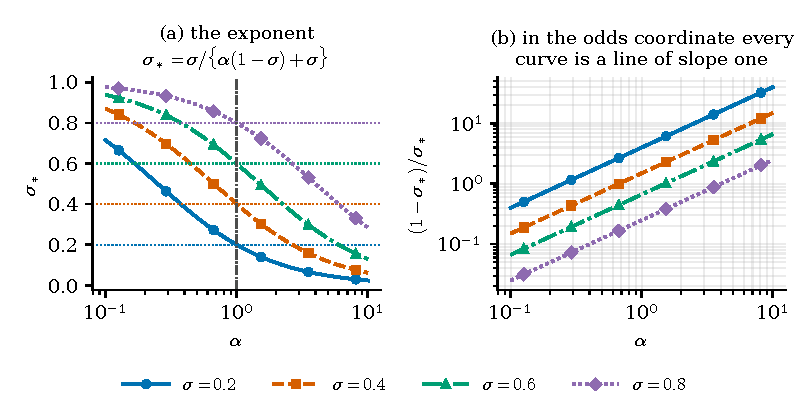
\includegraphics[width=\textwidth]{figures/py_fig-exponent.pdf}
\caption{The exponent map. Left, $\sigma_*$ against $\alpha$ for four values of $\sigma$, with the
unweighted values dotted and $\alpha = 1$ marked. Right, the same information in the odds
coordinate: every curve becomes a line of slope one through \eqref{py:eq:odds}, which is why two
different $(\sigma,\alpha)$ pairs with the same $\alpha(1-\sigma)/\sigma$ give the same exponent.}
\label{py:fig:exponent}
\end{figure}

\begin{figure}[t]
\centering
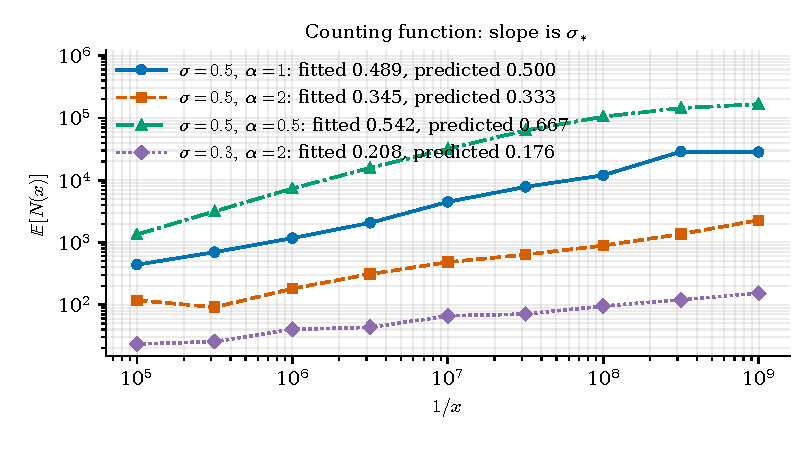
\includegraphics[width=\textwidth]{figures/py_fig-counting.pdf}
\caption{Counting functions of the induced frequencies over four decades in $x$, on log log axes.
The slope is $\sigma_*$. Fitted and predicted values are in the legend; the pair
$(\sigma,\alpha) = (0.5,1)$ and $(0.3,2)$ shows how far the exponent can move.}
\label{py:fig:counting}
\end{figure}

Figure~\ref{py:fig:counting} shows the exponent directly, by fitting the slope of
$\log \Ex[N(x)]$ on $\log(1/x)$ over the range where the truncated stick is still exact. The legend fits are
close for $\sigma = 0.5$ with $\alpha = 1$ and $2$ and rough for the other two curves ($0.542$ against $0.667$ and
$0.208$ against $0.176$).
Table~\ref{py:tab:exponent} collects a wider set, including the control $\alpha = 1$ where the answer
must be $\sigma$, and two rows sharing a $\sigma_*$ through \eqref{py:eq:odds}.

\begin{table}[t]
\centering
\caption{The exponent $\sigma_*$, predicted and fitted. Fitted values are the slope of
$\log \Ex[N(x)]$ on $\log(1/x)$ over a window above the truncation floor of a $2\times10^{6}$ stick
approximation, over $40$ replicates. The first and last rows have $\alpha(1-\sigma)/\sigma = 1$ and
so share an exponent.}
\label{py:tab:exponent}
\begin{adjustbox}{max width=\textwidth}
\begin{tabular}{rrrrr}
\toprule
$\sigma$ & $\theta$ & $\alpha$ & predicted $\sigma_*$ & fitted \\
\midrule
$0.5$  & $1$ & $1$    & $0.5000$ & $0.4996$ \\
$0.5$  & $1$ & $2$    & $0.3333$ & $0.3331$ \\
$0.5$  & $1$ & $0.5$  & $0.6667$ & $0.6669$ \\
$0.3$  & $1$ & $2$    & $0.1765$ & $0.1763$ \\
$0.7$  & $0$ & $3$    & $0.4375$ & $0.4360$ \\
$0.6$  & $1$ & $1.5$  & $0.5000$ & $0.5005$ \\
\bottomrule
\end{tabular}
\end{adjustbox}
\end{table}

\subsection{The layout does not change the exponent}
\label{py:sec:layout}

In the one parameter theory the arrangement of the atoms is decisive for the constant term and
irrelevant for the leading order. The same is true here, and for a reason that is visible in one
line.

\begin{proposition}
\label{py:prop:layout}
Lay the $\PD(\sigma,\theta)$ atoms in decreasing rather than size biased order and sample with
$f_\alpha$. Then $\log K_n/\log n \to \sigma_*$, the same exponent as in
Proposition~\ref{py:prop:pyimage}.
\end{proposition}

\begin{proof}
The ranked atoms of $\PD(\sigma,\theta)$ satisfy $V_{(k)}k^{1/\sigma} \to T$ a.s.\ for a positive
random $T$, so the ranked tail sums satisfy
\[
R_k = \sum_{i>k}V_{(i)} \;\asymp\; \int_k^\infty T u^{-1/\sigma}du
\;=\; \frac{\sigma T}{1-\sigma}\,k^{-(1-\sigma)/\sigma},
\]
which is the same power of $k$ as the size biased residual of Proposition~\ref{py:prop:pyimage}. Since
Lemma~\ref{py:lem:pit} makes the induced frequencies a function of the tail sums alone, and since the
decreasing layout case of the proof of Proposition~\ref{py:prop:index}, with $G(r) = r^{\alpha}$ and $\rho = \alpha$, uses only that power and the decay $V_{(k)}/R_{k-1} \sim \beta/k$, not the constant, the
conclusion is unchanged.
\end{proof}

Two remarks. First, this is not a triviality even though the proof is short: the two layouts have
genuinely different tail sum \emph{processes}, and what the argument uses is only that they share a
power. Second, the constant is a different matter. In the size biased layout the residual is a product of independent factors, so $M$ is the limit of
a normalised random walk. In the decreasing layout the tail sums are neither independent nor Markov
in any convenient sense, and the analogue of Lemma~\ref{py:lem:MS} would need the joint law of the
ranked atoms. This is exactly the split found in
the one parameter case, where the leading order is layout free and the constant is known in closed
form only in the size biased layout. Everything in Section~\ref{py:sec:diversity} should therefore be
read as a size biased statement.

\section{The diversity is a power of the unweighted diversity}
\label{py:sec:diversity}

Under $\PD(\sigma,\theta)$ the ratio $K_n/n^{\sigma}$ converges almost surely to the
$\sigma$ diversity $S = S_{\sigma,\theta}$, a Mittag Leffler variable with
\begin{equation}
\Ex[S^{p}] \;=\; \frac{\Gamma(\theta+1)\,\Gamma(\theta/\sigma+p+1)}
{\Gamma(\theta/\sigma+1)\,\Gamma(\theta+p\sigma+1)} ,
\qquad p > -1-\theta/\sigma .
\label{py:eq:mlmoments}
\end{equation}
Proposition~\ref{py:prop:pyimage} gives the exponent of the weighted problem but says nothing about
the limit of $K_n n^{-\sigma_*}$. In fact the two limits are the same random variable in disguise,
and the route to that goes through an identity worth recording on its own.

\begin{lemma}
\label{py:lem:MS}
With $M = \lim_k \widetilde R_k k^{(1-\sigma)/\sigma}$ as in Proposition~\ref{py:prop:pyimage},
\[
S \;=\; \Big(\frac{M}{\sigma}\Big)^{\sigma}
\qquad\text{almost surely.}
\]
\end{lemma}

\begin{proof}
Represent the stick fractions through independent Gamma variables,
$B_k = \Gamma_k/(\Gamma_k+\Gamma'_k)$ with $\Gamma_k \sim \Gamma(1-\sigma,1)$ and
$\Gamma'_k \sim \Gamma(\theta+k\sigma,1)$, all independent. Then
\[
p_k \;=\; \widetilde R_{k-1}B_k
\;=\; \widetilde R_{k-1}\,\frac{\Gamma_k}{\Gamma_k+\Gamma'_k}
\;=\; \frac{M}{\sigma}\,\Gamma_k\,k^{-1/\sigma}\,\varepsilon_k,
\qquad
\varepsilon_k := \frac{\widetilde R_{k-1}k^{\beta}}{M}\cdot\frac{k\sigma}{\Gamma_k+\Gamma'_k}.
\]
The first factor of $\varepsilon_k$ tends to $1$ almost surely by \eqref{py:eq:envelope}. For the
second, $\Gamma'_k$ has mean $\theta+k\sigma$ and a Gamma tail, so
$\Pr(|\Gamma'_k/(k\sigma) - 1| > \eta) \le 2e^{-c(\eta)k}$ is summable and
$\Gamma'_k/(k\sigma) \to 1$ almost surely; since $\Gamma_k = O(\log k)$ almost surely by the same
summability, $k\sigma/(\Gamma_k+\Gamma'_k) \to 1$ as well. Hence for every $\eta > 0$ there is an
almost surely finite $k_0$ with $1-\eta \le \varepsilon_k \le 1+\eta$ for $k \ge k_0$.

Fix $\eta$ and write $c_\pm = \sigma x/\{(1\mp\eta)M\}$. For $k \ge k_0$,
\[
\mathbf{1}\{\Gamma_k > c_+k^{1/\sigma}\} \;\le\; \mathbf{1}\{p_k > x\} \;\le\;
\mathbf{1}\{\Gamma_k > c_-k^{1/\sigma}\},
\]
so $N(x)$ is sandwiched, up to the $k_0$ early terms, between two sums
$N_\pm(x) = \sum_{k \ge k_0}\mathbf{1}\{\Gamma_k > c_\pm k^{1/\sigma}\}$ of independent indicators.
Their means are
\[
\Lambda_\pm(x) = \sum_{k\ge k_0}\Pr\big(\mathcal{G} > c_\pm k^{1/\sigma}\big)
\;\sim\; \int_0^\infty \Pr\big(\mathcal{G} > c_\pm u^{1/\sigma}\big)du
\;=\; c_\pm^{-\sigma}\,\Ex[\mathcal{G}^{\sigma}]
\quad (x \downarrow 0),
\]
the last step by the substitution $t = c_\pm u^{1/\sigma}$ and the identity
$\sigma\int_0^\infty t^{\sigma-1}\Pr(\mathcal{G}>t)\,dt = \Ex[\mathcal{G}^{\sigma}]$. Since
$\Var N_\pm \le \Lambda_\pm$ and $\Lambda_\pm(x) \to \infty$, Kolmogorov's criterion along
$x_j = (1+\delta)^{-j}$ gives $N_\pm(x_j)/\Lambda_\pm(x_j) \to 1$ almost surely, and monotonicity of $N$ in
$x$ extends this to all $x \downarrow 0$ up to a factor $(1+\delta)^{\pm\sigma}$, which is released as $\delta \downarrow 0$. Therefore
\[
(1-\eta)^{\sigma} \;\le\; \liminf_{x\downarrow0}\frac{x^{\sigma}N(x)}{(M/\sigma)^{\sigma}\Ex[\mathcal{G}^{\sigma}]}
\;\le\; \limsup_{x\downarrow0}\frac{x^{\sigma}N(x)}{(M/\sigma)^{\sigma}\Ex[\mathcal{G}^{\sigma}]}
\;\le\; (1+\eta)^{\sigma},
\]
and $\eta$ was arbitrary. For a $\Gamma(1-\sigma,1)$ variable
$\Ex[\mathcal{G}^{p}] = \Gamma(1-\sigma+p)/\Gamma(1-\sigma)$, so $\Ex[\mathcal{G}^{\sigma}] =
1/\Gamma(1-\sigma)$ and $x^{\sigma}N(x) \to (M/\sigma)^{\sigma}/\Gamma(1-\sigma)$ almost surely.
Karlin's occupancy correspondence, $K_n n^{-\sigma} \to \Gamma(1-\sigma)\lim x^{\sigma}N(x)$,
multiplies by $\Gamma(1-\sigma)$ and the two factors cancel.
\end{proof}

That the $\Gamma$ factors cancel is the reason the rest of this section is clean. The
$\sigma$ diversity is a deterministic power of the stick envelope with no constant left over, so
$M = \sigma S^{1/\sigma}$ can be substituted wherever the envelope appears. Since everything downstream rests on the identity, we checked it directly: estimating $M$ from the tail of the
stick and $S$ from the counting function on the same realisations, the ratio
$S/(M/\sigma)^{\sigma}$ has mean $0.9995$, $1.0020$, $0.9970$ and $0.9991$ at
$(\sigma,\theta) = (0.5,1)$, $(0.3,1)$, $(0.6,0)$ and $(0.5,2)$, over $80$ replicates with
$4\times10^{5}$ sticks.

\begin{proposition}
\label{py:prop:power}
Write $S_*$ for the almost sure limit of $K_n n^{-\sigma_*}$ under the weighted paintbox. Then
\begin{equation}
S_* \;=\; C\, S^{\kappa} \quad\text{almost surely},
\qquad
\kappa \;=\; \frac{\alpha\sigma_*}{\sigma} \;=\; \frac{\alpha}{\alpha(1-\sigma)+\sigma},
\label{py:eq:power}
\end{equation}
for a constant $C = C(\sigma,\alpha)$.
\end{proposition}

\begin{proof}
Both problems inherit the same envelope $M$: the unweighted frequencies satisfy
$p_k \asymp (M/\sigma)k^{-1/\sigma}$ and the weighted ones
$p'_k \asymp (\alpha M^{\alpha}/\sigma)k^{-1/\sigma_*}$. Counting as in Lemma~\ref{py:lem:MS} gives
$x^{\sigma}N(x) \to Z$ and $x^{\sigma_*}N_*(x) \to Z_*$ almost surely, with $Z$ and $Z_*$ each a
deterministic function of the single random variable $M$. Eliminating $M$ and applying Karlin's
correspondence to both gives \eqref{py:eq:power}, with the exponent
$\alpha\sigma_*/\sigma = \kappa$ read off the two envelopes.
\end{proof}

\begin{proposition}
\label{py:prop:constant}
In \eqref{py:eq:power},
\begin{equation}
C \;=\; \alpha^{\sigma_*}\,\sigma^{(\alpha-1)\sigma_*}\,
\frac{\Gamma(1-\sigma_*)\,\Gamma(1-\sigma+\sigma_*)}{\Gamma(1-\sigma)} .
\label{py:eq:C}
\end{equation}
In particular $C$ does not depend on $\theta$, and $C = 1$ at $\alpha = 1$.
\end{proposition}

\begin{proof}
The weighted frequencies are
$p'_k = \widetilde R_{k-1}^{\alpha}\{1-(1-B_k)^{\alpha}\}$. Since $B_k \to 0$ almost surely and
$\{1-(1-B)^{\alpha}\}/(\alpha B) \to 1$ as $B \to 0$, the argument of Lemma~\ref{py:lem:MS} applies
verbatim with $\widetilde R_{k-1}^{\alpha}$ in place of $\widetilde R_{k-1}$ and one further
factor, tending to one, absorbed into $\varepsilon_k$: for $k \ge k_0$,
\[
p'_k \;=\; \frac{\alpha M^{\alpha}}{\sigma}\,\Gamma_k\,k^{-1/\sigma_*}\,\varepsilon'_k,
\qquad 1-\eta \le \varepsilon'_k \le 1+\eta,
\]
with the same Gamma variables $\Gamma_k$, because they come from the same sticks, and with
$\alpha\beta+1 = 1/\sigma_*$. The sandwich then gives, with $\sigma_*$ in place of $\sigma$ in the
substitution,
\[
x^{\sigma_*}N_*(x) \;\longrightarrow\;
\Big(\frac{\alpha M^{\alpha}}{\sigma}\Big)^{\sigma_*}
\Ex[\mathcal{G}^{\sigma_*}]
\;=\;
\Big(\frac{\alpha M^{\alpha}}{\sigma}\Big)^{\sigma_*}
\frac{\Gamma(1-\sigma+\sigma_*)}{\Gamma(1-\sigma)}
\quad\text{almost surely,}
\]
and $S_* = \Gamma(1-\sigma_*)$ times that. Substituting $M = \sigma S^{1/\sigma}$ from
Lemma~\ref{py:lem:MS} and using $\alpha\sigma_*/\sigma = \kappa$ gives \eqref{py:eq:C}.
\end{proof}

\begin{corollary}
\label{py:cor:moments}
$\Ex[S_*^{p}] = C^{p}\,\Ex[S^{\kappa p}]$ for $p > -(1+\theta/\sigma)/\kappa$, with the right side given by
\eqref{py:eq:mlmoments} at $\kappa p$. Comparing that expression, as a function of $p$, with \eqref{py:eq:mlmoments} shows it is of
Mittag Leffler form only when $\kappa = 1$, that is only when $\alpha = 1$: the gamma factors in
$p$ are spaced by $1/\kappa$ on one side and by $1$ on the other.
\end{corollary}

Two comments. First, that $\theta$ is absent from \eqref{py:eq:C} is the second appearance of the
phenomenon noted after Proposition~\ref{py:prop:pyimage}. It does not mean $\theta$ is irrelevant to
the weighted problem: it enters through the law of $S$ itself, by \eqref{py:eq:mlmoments}. What it
means is that the \emph{map} from the unweighted diversity to the weighted one is free of $\theta$,
so ascertainment acts on the diversity by a transformation fixed by $\sigma$ and $\alpha$ alone.
Second, the Mittag Leffler family is not closed under powers, so Corollary~\ref{py:cor:moments} is a
second sense in which ascertainment leaves the standard families, and it matches the first:
exactness fails at the level of the law, and closure fails at the level of the diversity.

\begin{figure}[t]
\centering
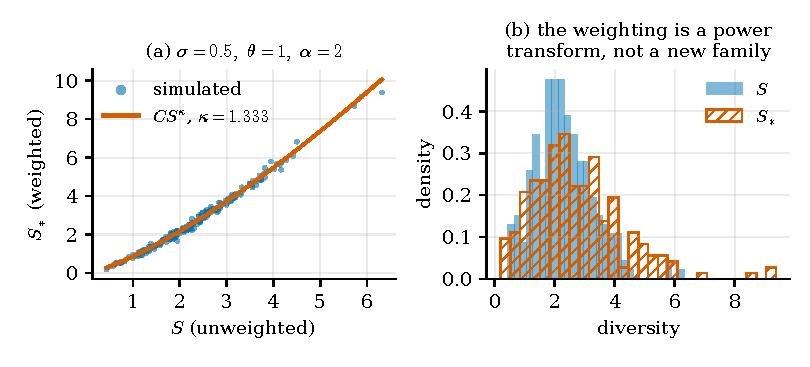
\includegraphics[width=\textwidth]{figures/py_fig-diversity.pdf}
\caption{The diversity map at $\sigma = 0.5$, $\theta = 1$, $\alpha = 2$, so $\kappa = 4/3$. Left,
the weighted diversity against the unweighted one on common stick realisations, with the predicted
curve $CS^{\kappa}$ of \eqref{py:eq:power} and \eqref{py:eq:C} overlaid; the identity is pathwise, not
merely in distribution. Right, the two densities: the weighting widens the diversity and
changes its shape, because a power of a Mittag Leffler variable is not Mittag Leffler.}
\label{py:fig:diversity}
\end{figure}

Table~\ref{py:tab:constant} checks \eqref{py:eq:C} against simulation. What is tested is the ratio
$Z_*/Z^{\kappa}$, estimated on common stick realisations so the comparison is pathwise; the last
column is the relative standard deviation of that ratio across replicates, which measures how
nearly \eqref{py:eq:power} holds pathwise rather than in mean.

\begin{table}[t]
\centering
\caption{The constant of \eqref{py:eq:C} tested through the ratio
$Z_*/Z^{\kappa} = C\,\Gamma(1-\sigma)^{\kappa}/\Gamma(1-\sigma_*)$, predicted and simulated, using $2\times10^{6}$ sticks at
level $x = 10^{-7}$ over $60$ replicates with $Z$ and $Z_*$ computed on the same realisation. The
$\alpha = 1$ row is exact; the last row tests the $\theta$ independence of \eqref{py:eq:C}.}
\label{py:tab:constant}
\begin{adjustbox}{max width=\textwidth}
\begin{tabular}{rrrrrrr}
\toprule
$\sigma$ & $\theta$ & $\alpha$ & $\sigma_*$ & predicted & simulated & rel.\ s.d.\\
\midrule
$0.5$ & $1$ & $2$   & $0.3333$ & $1.3661$ & $1.3588$ & $0.065$\\
$0.4$ & $1$ & $2$   & $0.2500$ & $1.1623$ & $1.1559$ & $0.101$\\
$0.6$ & $1$ & $1.5$ & $0.5000$ & $1.4058$ & $1.4034$ & $0.019$\\
$0.5$ & $1$ & $1$   & $0.5000$ & $1.0000$ & $1.0000$ & $0.000$\\
$0.5$ & $2$ & $2$   & $0.3333$ & $1.3661$ & $1.3650$ & $0.050$\\
\bottomrule
\end{tabular}
\end{adjustbox}
\end{table}

The first three rows agree to within Monte Carlo error and the $\alpha = 1$ row is exact, as it
must be. Doubling $\theta$ moves the simulated constant by less than half a percent, well within
the sampling error at this $x$.

\begin{remark}
The proofs of Lemma~\ref{py:lem:MS} and Proposition~\ref{py:prop:constant} use two facts about the
Gamma representation of the sticks: that the large shape Gamma variable concentrates exponentially
fast, and that the resulting count is a sum of independent indicators to which Kolmogorov's
criterion applies. Neither step is delicate, and the sandwich makes the nonuniformity of the
approximations harmless, since it costs only a factor $(1\pm\eta)^{\sigma}$ that is released at the
end. The one place where care is needed is the passage from a geometric grid $x_j = (1+\delta)^{-j}$, with $\delta \downarrow 0$ at the end, to all $x$, and there the
monotonicity of $N$ does the work.
\end{remark}

\section{The coincidence theory collapses}
\label{py:sec:coincidence}

The other half of the one parameter theory asks for the probability that no two intervals receive
the same number of points. Under $\ESF(\vartheta)$ that probability tends to
$e^{-\gamma\vartheta}/\Gamma(1+\vartheta)$, and the whole analysis turns on the small frequencies
forming a point process of intensity $\vartheta u^{-1}du$, which is scale invariant. None of it
survives $\sigma > 0$, and the reason is the same intensity.

\begin{proposition}
\label{py:prop:nocoin}
For a $\PD(\sigma,\theta)$ paintbox with $\sigma > 0$, and for every weight $f$ of positive index in
the sense of Proposition~\ref{py:prop:index}, in particular every $f_\alpha$, the probability that all
occupied intervals receive distinct counts tends to zero.
\end{proposition}

Under $f_\alpha$ the small frequencies have intensity proportional to $x^{-1-\sigma_*}dx$, and
under any weight of positive index in the sense of Proposition~\ref{py:prop:index} their counting function is regularly varying with index $-\sigma_*$, again strictly negative. It is
never $\vartheta u^{-1}du$. So $A_j/K_n \to q_j(\sigma_*) > 0$ for each fixed $j$
(Section~\ref{py:sec:survives}), and since $K_n \to \infty$, in particular $A_1 \to \infty$: there are eventually many singletons and ties are certain. A
power intensity is also not scale invariant, so the invariance result of the one parameter theory,
that any weight continuous and positive at the right endpoint leaves the constant untouched, has
nothing to act on either.

Figure~\ref{py:fig:coincidence} shows both halves. On the left, $\Ex[A_1]$ is bounded at $\sigma = 0$
and grows like $n^{\sigma}$ beyond it; the slopes on log log axes are the exponents. On the right,
the probability that all abundances are distinct approaches its limit $e^{-\gamma}$ for the
one parameter case and falls to zero for every $\sigma > 0$, faster the larger $\sigma$ is.

\begin{figure}[t]
\centering
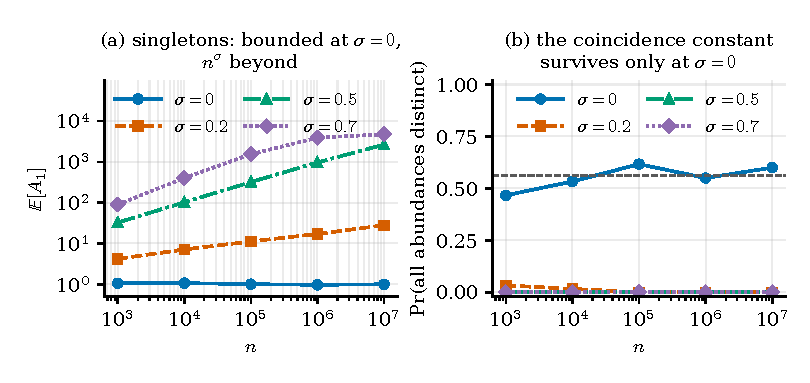
\includegraphics[width=\textwidth]{figures/py_fig-coincidence.pdf}
\caption{Why the coincidence constant is a one parameter phenomenon. Left, the expected number of
singletons: bounded at $\sigma = 0$, growing like $n^{\sigma}$ for $\sigma > 0$. Right, the
probability that no two intervals receive the same number of points; the dashed line is
$e^{-\gamma} = 0.5615$, the $\ESF(1)$ limit. Uniform sampling, $\alpha = 1$, throughout.}
\label{py:fig:coincidence}
\end{figure}

That is a negative result but a clarifying one. The two questions one is naturally led to ask, the
first order profile and the coincidence law, are not two aspects of a single theory. The first
generalises with a change of coordinate; the second is specific to $\sigma = 0$ and to the scale
invariance of the logarithmic intensity.

\section{Estimating the discount parameter from a biased sample}
\label{py:sec:estimation}

The statistical content of Proposition~\ref{py:prop:pyimage} is a bias with an exact inverse. A
practitioner who estimates the discount parameter by the growth of the number of types, and whose
sample is drawn with effort profile $f_\alpha$ rather than uniformly, does not estimate $\sigma$.
He estimates $\sigma_*$, and by \eqref{py:eq:odds} the map is invertible.

\begin{corollary}
\label{py:cor:correct}
If $\alpha$ is known by design and $\hat\sigma_*$ is any consistent estimator of the exponent from
the weighted sample, then
\begin{equation}
\hat\sigma \;=\; \frac{\alpha\hat\sigma_*}{\alpha\hat\sigma_* + 1 - \hat\sigma_*}
\label{py:eq:correct}
\end{equation}
is consistent for $\sigma$. Equivalently, in the odds coordinate the correction is a division by
$\alpha$.
\end{corollary}

\begin{proof}
Invert $\sigma_* = \sigma/\{\alpha(1-\sigma)+\sigma\}$, or equivalently divide
$(1-\sigma_*)/\sigma_*$ by $\alpha$ and solve.
\end{proof}

Three estimators of $\sigma_*$ are now available, and they are not equivalent. The exponent
estimator $\log K_n/\log n$ is the obvious one and the worst: it converges only logarithmically,
and at $n = 10^{6}$ with $\log n = 13.8$ an $O(1)$ error in $\log K_n$ is already an error of
order $0.07$ in the exponent. The two spectrum estimators, $1-2A_2/A_1$ from
Corollary~\ref{py:cor:spectrum} and $A_1/K_n$ from Corollary~\ref{py:cor:singleton}, are ratios of counts
at the same $n$ and converge at the rate the counts do.

Figure~\ref{py:fig:estimation} compares them at $\sigma = 0.5$, $n = 10^{6}$. For $\alpha \ge 1$, the fading effort of a tiring collector and the common case in practice, the
two spectrum estimators are close to exact. At $\alpha = 1, 2, 4$ they return $0.500, 0.341, 0.199$
and $0.500, 0.344, 0.201$ against targets $0.500, 0.333, 0.200$; $\log K_n/\log n$ returns
$0.547, 0.397, 0.263$. For $\alpha < 1$ the picture appears to reverse: at $\alpha = 0.25$, where $\sigma_* = 0.8$, the
spectrum estimators read $0.61$ and $0.67$ while the exponent estimator reads $0.798$. That
comparison is an artefact and should not be believed, for the reason set out in
Section~\ref{py:sec:truncation}: a persistent weight makes the truncated stick a poor approximation, and
the omitted mass depresses the spectrum estimators specifically. Raising the stick count at fixed
$n$ moves $A_1/K_n$ steadily back towards $\sigma_*$. What the left panel shows for $\alpha < 1$ is
the limit of the simulation, not the limit of the estimator.

The right panel applies the correction. It is exact for all three in the limit, being the inverse
group element of Proposition~\ref{py:prop:group}, so what the panel shows is the accuracy of the
underlying estimator and nothing else. The spectrum estimators recover $\sigma = 0.5$ to within
about $0.01$ for $\alpha \ge 1$ and lose accuracy as $\alpha$ falls; the exponent estimator drifts across
the whole range, from $0.50$ to $0.59$, its errors partly cancelling in the correction. In practice
one would use $A_1/K_n$, check it against $1-2A_2/A_1$, and treat disagreement between them as a
warning that the sample is too small for the stable regime to have set in.

\begin{figure}[t]
\centering
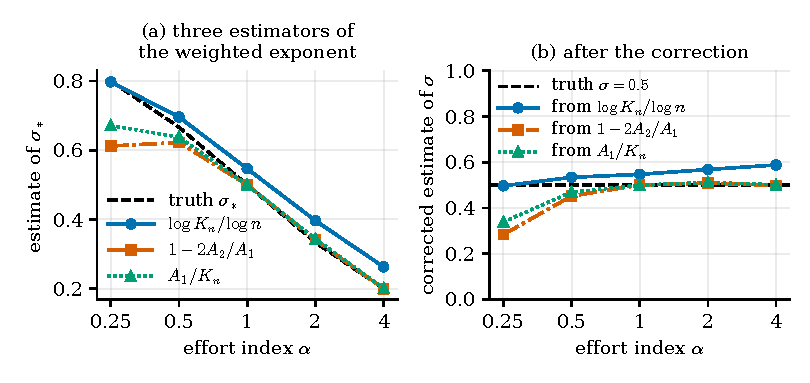
\includegraphics[width=\textwidth]{figures/py_fig-estimation.pdf}
\caption{Estimating $\sigma = 0.5$ from a sample drawn with effort profile $f_\alpha$, at
$n = 10^{6}$ over $24$ replicates. Left, three estimators of the weighted exponent against its true
value. Right, the same three after the correction \eqref{py:eq:correct}, whose target is the dashed
line. The spectrum estimators are near exact for $\alpha \ge 1$ and degrade as $\sigma_*$
approaches one; the exponent estimator is mediocre everywhere.}
\label{py:fig:estimation}
\end{figure}

\subsection{The effort profiles form a group, and the odds coordinate linearises it}
\label{py:sec:group}

Write $T_\alpha$ for the map on the discount parameter induced by the weight $f_\alpha$, so
$T_\alpha(\sigma) = \sigma/\{\alpha(1-\sigma)+\sigma\}$.

\begin{proposition}
\label{py:prop:group}
$T_\alpha \circ T_{\alpha'} = T_{\alpha\alpha'}$ for all $\alpha, \alpha' > 0$, with
$T_1 = \mathrm{id}$ and $T_\alpha^{-1} = T_{1/\alpha}$. The family $\{T_\alpha\}$ is therefore a
one parameter group isomorphic to the multiplicative positive reals, and \eqref{py:eq:odds} is the
coordinate in which the action is multiplication.
\end{proposition}

\begin{proof}
Composition of weights is composition of the maps $G$, and $r^{\alpha'} \mapsto (r^{\alpha'})^{\alpha}
= r^{\alpha\alpha'}$. In the odds coordinate $\omega = (1-\sigma)/\sigma$ the action is
$\omega \mapsto \alpha\omega$ by \eqref{py:eq:odds}, and multiplication composes.
\end{proof}

The group property is a consistency check on the whole framework, and it says something about
design. Applying two effort profiles in succession, a fading pass and then a persistent one, is the
same as applying a single profile with the product index; there is no path dependence and no
interaction. It also means the correction \eqref{py:eq:correct} is exactly the inverse group element,
which is why it is exact and not merely first order.

The exponent inherits the group structure: writing $\kappa(\sigma,\alpha)$ for the power in
\eqref{py:eq:power},
\begin{equation}
\kappa(\sigma,\alpha\alpha') \;=\; \kappa(\sigma,\alpha')\,\kappa\big(T_{\alpha'}(\sigma),\alpha\big)
\label{py:eq:kappacomp}
\end{equation}
identically, which we verified at forty five parameter triples to machine precision.

The constant does not, and the failure is instructive rather than embarrassing. One might expect
the cocycle relation
\begin{equation}
C(\sigma,\alpha\alpha') \;\overset{?}{=}\; C\big(T_{\alpha'}(\sigma),\alpha\big)\,
C(\sigma,\alpha')^{\kappa(T_{\alpha'}(\sigma),\alpha)},
\label{py:eq:cocycle}
\end{equation}
obtained by applying \eqref{py:eq:power} twice. It fails, by the amounts computed below. The reason is Theorem~\ref{py:thm:rigid}. The second application of
\eqref{py:eq:power} is only legitimate if the intermediate object is a $\PD(\sigma',\theta')$ system,
and it is not: after the first weighting the subdivision is the residual allocation model
\eqref{py:eq:image}, which lies outside the Ewens Pitman family. The exponent survives the detour
because it depends only on the power of $k$ in the tail sums, which \eqref{py:eq:image} shares with a
genuine two parameter law; the constant does not, because it depends on the law of the stick
fractions, which \eqref{py:eq:image} does not share.

So the size of the gap in \eqref{py:eq:cocycle} is a quantitative measure of how far the image is from
the family it left, and it is a measure computable in closed form from \eqref{py:eq:C}, with no
simulation. It is zero when $\alpha = 1$ or $\alpha' = 1$, and, at $\sigma = 0.65$, largest when both weights fade:
about four percent at $(\sigma,\alpha,\alpha') = (0.65, 2, 3)$, seven percent at $(0.65, 3, 3)$ and eleven percent at $(0.65, 4, 4)$. It is negative when one weight fades and the other persists, and small when both persist, $0.12$ percent at $(0.65, 0.5, 0.5)$. That is a second and
sharper reading of Theorem~\ref{py:thm:rigid}: the family is not merely unpreserved, it is
unpreserved by an amount one can compute.

\subsection{Moments of the weighted diversity}
\label{py:sec:moments}

Corollary~\ref{py:cor:moments} makes every moment explicit, and the numbers show that the weighting
does not merely shift the diversity but changes its shape.
Table~\ref{py:tab:moments} gives the mean, standard deviation and coefficient of variation of $S_*$ at
$\sigma = 0.5$, $\theta = 1$, computed from \eqref{py:eq:mlmoments} and \eqref{py:eq:C} with no
simulation.

\begin{table}[t]
\centering
\caption{Moments of the weighted $\sigma$ diversity at $\sigma = 0.5$, $\theta = 1$, from
$\Ex[S_*^{p}] = C^{p}\Ex[S^{\kappa p}]$. The row $\alpha = 1$ is the Mittag Leffler law itself.}
\label{py:tab:moments}
\begin{adjustbox}{max width=\textwidth}
\begin{tabular}{rrrrrrr}
\toprule
$\alpha$ & $\sigma_*$ & $\kappa$ & $C$ & $\Ex[S_*]$ & $\mathrm{sd}[S_*]$ & c.v.\\
\midrule
$0.25$ & $0.800$ & $0.400$ & $1.1623$ & $1.572$ & $0.283$ & $0.180$\\
$0.5$  & $0.667$ & $0.667$ & $1.1129$ & $1.875$ & $0.544$ & $0.290$\\
$1$    & $0.500$ & $1.000$ & $1.0000$ & $2.257$ & $0.952$ & $0.422$\\
$2$    & $0.333$ & $1.333$ & $0.8624$ & $2.654$ & $1.465$ & $0.552$\\
$4$    & $0.200$ & $1.600$ & $0.7423$ & $2.962$ & $1.944$ & $0.656$\\
\bottomrule
\end{tabular}
\end{adjustbox}
\end{table}

The coefficient of variation moves by a factor of nearly four across the range. A fading effort
profile, $\alpha > 1$, raises the diversity to a power greater than one and so stretches its upper
tail: the type count becomes both larger in mean, on the $n^{\sigma_*}$ scale, and much more
variable between replicate surveys. A persistent profile does the reverse and produces an
artificially stable diversity. Either way an analyst who fits a Mittag Leffler law to replicate
surveys, as the two parameter model instructs, will find it does not fit, and the reason is not the
model but the sampling.

\section{The joint law of the counts}
\label{py:sec:joint}

Everything so far concerns $K_n$ and the diversity. The abundance spectrum $(A_1,A_2,\dots)$ is a
finer object, and in the one parameter case it is the one that carries the interesting structure:
there the counts converge to \emph{independent} Poisson variables with means $\vartheta/j$, a
genuinely infinite dimensional limit. Two points of precision are owed here, both of which Warren
Ewens insisted on. At finite $n$ the $A_j$ under $\ESF(\vartheta)$ are \emph{not} independent: the
exact statement is the conditioning relation, that $(A_1,\dots,A_n)$ has the law of independent
$Z_j \sim \mathrm{Poisson}(\vartheta/j)$ conditioned on $\sum_j jZ_j = n$
\citep{py:arratia2003}, and independence emerges only in the limit, for
$(A_1,\dots,A_b)$ with $b$ fixed as $n \to \infty$. Likewise the coincidence constant
$e^{-\gamma\vartheta}/\Gamma(1+\vartheta)$ is the limiting value of the probability that all
abundances are distinct and not its value at any finite $n$. For $\sigma > 0$ the answer is the
opposite, and simpler.

\begin{proposition}
\label{py:prop:joint}
Under the weighted paintbox with $\sigma > 0$, for each fixed $j$,
\begin{equation}
\frac{A_j}{n^{\sigma_*}} \;\longrightarrow\; q_j(\sigma_*)\,S_* ,
\qquad
q_j(\sigma) \;=\; \frac{\sigma\,\Gamma(j-\sigma)}{\Gamma(1-\sigma)\,j!},
\label{py:eq:joint}
\end{equation}
jointly in $j$ and almost surely, with $S_*$ the limit of Proposition~\ref{py:prop:power}.
\end{proposition}

\begin{proof}
Poissonise and condition on the frequencies. With $\pi_j(u) = u^{j}e^{-u}/j!$ we have
$\Ex[A_j \mid P] = \sum_k \pi_j(np_k)$, and the induced frequencies have counting function
$N(x) \sim Z_* x^{-\sigma_*}$, so the number of them in $(x,x+dx)$ is
$Z_*\sigma_* x^{-\sigma_*-1}dx$. Hence
\[
\begin{aligned}
\sum_k \pi_j(np_k) &\;\approx\; \int_0^\infty \pi_j(nx)\,Z_*\sigma_* x^{-\sigma_*-1}dx\\
&\;=\; Z_*\sigma_* n^{\sigma_*}\frac{1}{j!}\int_0^\infty u^{\,j-\sigma_*-1}e^{-u}du
\;=\; Z_*\,\frac{\sigma_*\Gamma(j-\sigma_*)}{j!}\,n^{\sigma_*} .
\end{aligned}
\]
Since $S_* = \Gamma(1-\sigma_*)Z_*$, this is $q_j(\sigma_*)S_*n^{\sigma_*}$. The display is the
heuristic; the rigorous version is Lemma~\ref{py:lem:karlin} applied conditionally on the
frequencies, with $\gamma = \sigma_*$ and the constant slowly varying function $L \equiv Z_*$, which
is legitimate because $x^{\sigma_*}N_*(x) \to Z_*$ almost surely by the proof of
Proposition~\ref{py:prop:constant}. The lemma gives $A_j/n^{\sigma_*} \to \sigma_*\Gamma(j-\sigma_*)Z_*/j!$
almost surely for each $j$, and since countably many almost sure statements hold simultaneously,
the convergence is joint in $j$ with the same $S_*$ throughout.
\end{proof}

The limit is degenerate given $S_*$: every coordinate is a deterministic multiple of one random
variable. Two checks confirm the normalisation. At $j = 1$ the constant is $q_1 = \sigma_*$, so
$A_1/n^{\sigma_*} \to \sigma_* S_*$; and $\sum_{j\ge1}q_j(\sigma) = 1$ by the identity
$\sum_{j\ge1}\Gamma(j-\sigma)/j! = \Gamma(1-\sigma)/\sigma$, which recovers
$K_n/n^{\sigma_*} \to S_*$. The identity is the binomial series at its boundary. For $|x| \le 1$,
\[
(1-x)^{\sigma} \;=\; \sum_{j\ge0}\frac{(-\sigma)_j}{j!}\,x^{j}
\;=\; 1 + \sum_{j\ge1}\frac{\Gamma(j-\sigma)}{\Gamma(-\sigma)\,j!}\,x^{j},
\]
the series converging at $x = 1$ because its terms are of order $j^{-1-\sigma}$. Setting $x = 1$ gives
$\sum_{j\ge1}\Gamma(j-\sigma)/j! = -\Gamma(-\sigma) = \Gamma(1-\sigma)/\sigma$. The terms
$q_j(\sigma) = \sigma\Gamma(j-\sigma)/\{\Gamma(1-\sigma)j!\}$ are therefore a probability
distribution on $j \ge 1$, Sibuya's distribution, and Proposition~\ref{py:prop:joint} says that
the abundance of a randomly chosen observed type is asymptotically Sibuya distributed with
parameter $\sigma_*$. Its first terms are $q_1 = \sigma_*$, $q_2 = \sigma_*(1-\sigma_*)/2$ and
$q_3 = \sigma_*(1-\sigma_*)(2-\sigma_*)/6$.

Together the proposition and its normalisation give a prediction with no constant in it at all.

\begin{corollary}[The singleton fraction]
\label{py:cor:singleton}
$A_1/K_n \to \sigma_*$ almost surely. In a two parameter community the fraction of observed types
seen exactly once estimates the discount parameter directly; under a biased sample it estimates
$\sigma_*$, which Corollary~\ref{py:cor:correct} inverts.
\end{corollary}

\begin{proof}
Divide \eqref{py:eq:joint} at $j=1$, where $q_1(\sigma_*) = \sigma_*$, by
$K_n/n^{\sigma_*} \to S_*$; the random factor $S_*$ cancels.
\end{proof}

Notice how little this asks. No normalisation, no knowledge of $n$, no estimate of
$S_*$ or $\theta$: two numbers a survey already reports, the count of types and the count of types
seen once. At $n = 10^{8}$ simulation gives $A_1/K_n = 0.3326$ against $\sigma_* = 1/3$ and $0.1752$ against
$0.1765$. At $\sigma_* = 1/2$ the same simulation gives $0.4724$, which is not a property of the
estimator but of the simulation: raising the number of sticks from $3\times10^{5}$ to
$1.5\times10^{6}$ moves it to $0.4885$ and then $0.4953$. Section~\ref{py:sec:truncation} below says how many sticks are
needed, and why the answer is sometimes impossible.

\subsection{A dichotomy, and an estimator}

The contrast with $\sigma = 0$ is complete. There the spectrum converges to an infinite family of
independent Poisson variables, and no scaling makes it degenerate; the interesting questions are
about the joint law, which is where the coincidence probability of the one parameter theory lives.
Here the spectrum converges, after a single scaling, to a deterministic profile multiplied by one
random number. All the randomness in the abundance spectrum of a two parameter community is the
randomness of its diversity.

That degeneracy is a practical gift, because it makes the shape of the spectrum a deterministic
function of $\sigma_*$ alone, free of $S_*$, of $\theta$ and of $n$.

\begin{corollary}
\label{py:cor:spectrum}
For each $j \ge 2$,
\begin{equation}
\frac{A_j}{A_1} \;\longrightarrow\; \frac{\Gamma(j-\sigma_*)}{j!\,\Gamma(1-\sigma_*)} ,
\qquad\text{in particular}\qquad
\frac{A_2}{A_1} \;\longrightarrow\; \frac{1-\sigma_*}{2} .
\label{py:eq:spectrum}
\end{equation}
Hence $\hat\sigma_* = 1 - 2A_2/A_1$ is consistent for $\sigma_*$, and
$\hat\sigma = \alpha\hat\sigma_*/(\alpha\hat\sigma_*+1-\hat\sigma_*)$ by
Corollary~\ref{py:cor:correct} is consistent for $\sigma$.
\end{corollary}

\subsection{The bias of the singleton fraction}
\label{py:sec:rate}

How large must a survey be before $A_1/K_n$ can be trusted? The answer is: not very, and the
calculation is a Mellin transform.

\begin{proposition}
\label{py:prop:rate}
Suppose the induced frequencies follow the envelope $p_k = c\,k^{-1/\sigma_*}$ exactly, and write
$A = nc$. Then, as $A \to \infty$,
\[
\begin{gathered}
\Ex[A_1 \mid P] = \sigma_*\Gamma(1-\sigma_*)A^{\sigma_*} + O(A^{-\delta}),
\\
\Ex[K_n \mid P] = \Gamma(1-\sigma_*)A^{\sigma_*} - \tfrac12 + O(A^{-\delta}),
\end{gathered}
\]
for some $\delta > 0$, and consequently
\begin{equation}
\frac{\Ex[A_1\mid P]}{\Ex[K_n\mid P]} \;=\; \sigma_*\Big(1 + \frac{1}{2\,\Ex[K_n\mid P]}\Big) + o\!\left(\frac{1}{\Ex[K_n\mid P]}\right).
\label{py:eq:rate}
\end{equation}
\end{proposition}

\begin{proof}
For $f$ with Mellin transform $\tilde f(s) = \int_0^\infty f(u)u^{-s-1}du$, substituting
$v = Ak^{-1/\sigma_*}$ gives $\int_0^\infty f(Ak^{-1/\sigma_*})A^{-s-1}dA = k^{-s/\sigma_*}\tilde f(s)$,
so $\sum_{k\ge1} f(Ak^{-1/\sigma_*})$ has Mellin transform $\zeta(s/\sigma_*)\tilde f(s)$ and equals
$(2\pi i)^{-1}\int \zeta(s/\sigma_*)\tilde f(s)A^{s}ds$. Shifting the contour left collects
residues. For $A_1$ take $f(u) = ue^{-u}$, whose transform is $\Gamma(1-s)$; the only pole crossed
is that of $\zeta$ at $s = \sigma_*$, with residue $\sigma_*\Gamma(1-\sigma_*)A^{\sigma_*}$. For
$K_n$ take $f(u) = 1-e^{-u}$, whose transform is $\Gamma(1-s)/s$ on $0 < \Re s < 1$; here the
contour crosses the same pole, giving $\Gamma(1-\sigma_*)A^{\sigma_*}$, and additionally the pole
of $1/s$ at the origin, whose residue is $\zeta(0)\Gamma(1) = -\tfrac12$. Dividing and expanding
gives \eqref{py:eq:rate}.
\end{proof}

Two things follow. The deterministic bias is $O(1/K_n)$, whereas the sampling standard deviation of
$A_1/K_n$ is $O(K_n^{-1/2})$: at any sample size where the estimator has appreciable noise the bias
is invisible beside it, and there is no bias correction worth making. And the coefficient is
$\sigma_*/2$, so the bias is upward, not downward, which is worth saying because every deficit
of $A_1/K_n$ observed up to here has been downward and every one of them was truncation.

Simulating the deterministic envelope directly, with $4\times10^{7}$ frequencies and no random
sticks, isolates \eqref{py:eq:rate} from the difficulty of Section~\ref{py:sec:truncation}. At
$\sigma_* = 0.3$ the quantity $(A_1/K_n - \sigma_*)K_n$ equals $0.1500$ at $n = 10^{5}$, $10^{6}$
and $10^{7}$, against the predicted $\sigma_*/2 = 0.15$, to four decimal places at every sample
size. At $\sigma_* = 0.5$ it gives $0.249$ and $0.242$ against $0.25$ at the first two sample sizes.
At $\sigma_* = 0.7$ it fails, and fails worse as $n$ grows, for the reason \eqref{py:eq:trunc}
predicts: the envelope $k^{-1/0.7}$ has so heavy a tail that $4\times10^{7}$ frequencies do not
cover the range a sample of $10^{7}$ explores.

The doubleton ratio $1-2A_2/A_1$ is a better estimator than the exponent estimator of Section~\ref{py:sec:estimation} for the reason given there:
$\log K_n/\log n$ converges to $\sigma_*$ only logarithmically, whereas \eqref{py:eq:spectrum} is a
ratio of two counts at the same $n$ and converges at the rate the counts themselves do. It needs
neither $n$ nor any normalisation, only the number of singletons and the number of doubletons, both
of which a survey reports. At $\sigma_* \to 0$ it returns $A_2/A_1 \to 1/2$, which is the
one parameter value $\Ex[A_j] \propto 1/j$, so the estimator degrades gracefully to the boundary of
the family.

Table~\ref{py:tab:joint} tests \eqref{py:eq:joint} and \eqref{py:eq:spectrum} by Rao Blackwellised
simulation. The predicted and observed ratios $A_3/A_1$ and $A_4/A_1$ agree closely wherever the
truncated stick resolves the relevant range, and the estimator $1-2A_2/A_1$ recovers $\sigma_*$.
The last two rows are the same configuration at two truncation levels, and they show where the
residual error comes from. That configuration has $\alpha = 1/2$, so by the criterion
\eqref{py:eq:trunc} of Section~\ref{py:sec:truncation} below an honest simulation would need
$K \gg n^{2}$ sticks: $3\times10^{5}$ sticks at $n = 10^{8}$ are short by
some ten orders of magnitude and the estimator reads $-0.09$. Raising the stick count to
$2\times10^{6}$ and lowering $n$ to $10^{7}$ brings it to $0.578$ against a target of $0.667$, still
far inside the regime \eqref{py:eq:trunc} forbids. The deficit is ours and not the estimator's.

\begin{table}[t]
\centering
\caption{The spectrum profile \eqref{py:eq:joint} and the estimator \eqref{py:eq:spectrum}. Counts are
Rao Blackwellised, $\Ex[A_j\mid P] = \binom{n}{j}\sum_k p_k^j(1-p_k)^{n-j}$, over $40$
replicates at $n = 10^{8}$ with $3\times10^{5}$ sticks unless marked. The final row repeats the
fifth at $n = 10^{7}$ with $2\times10^{6}$ sticks.}
\label{py:tab:joint}
\begin{adjustbox}{max width=\textwidth}
\begin{tabular}{rrrrrrr}
\toprule
$\sigma$ & $\theta$ & $\alpha$ & $\sigma_*$ & $1-2A_2/A_1$
& $A_3/A_1$ pred/obs & $A_4/A_1$ pred/obs\\
\midrule
$0.5$ & $1$ & $1$   & $0.5000$ & $0.451$ & $0.125/0.138$ & $0.078/0.086$\\
$0.5$ & $1$ & $2$   & $0.3333$ & $0.331$ & $0.185/0.186$ & $0.124/0.125$\\
$0.3$ & $1$ & $2$   & $0.1765$ & $0.183$ & $0.250/0.248$ & $0.177/0.177$\\
$0.6$ & $0$ & $1.5$ & $0.5000$ & $0.473$ & $0.125/0.132$ & $0.078/0.082$\\
$0.5$ & $2$ & $0.5$ & $0.6667$ & $-0.090$ & $0.074/0.344$ & $0.043/0.236$\\
$0.5$ & $2$ & $0.5$ & $0.6667$ & $0.578$ & $0.074/0.094$ & $\cdot$ \\
\bottomrule
\end{tabular}
\end{adjustbox}
\end{table}

\begin{remark}
Proposition~\ref{py:prop:joint} also settles, negatively, a question one might ask by analogy with the
one parameter theory. There the interesting phenomenon is that the layout of the atoms changes the
joint law of the counts while leaving the profile $\Ex[A_j]$ alone. Here there is no room for such
an effect: by Proposition~\ref{py:prop:layout} the exponent is layout free, and by
\eqref{py:eq:joint} the whole spectrum is determined by the exponent and by $S_*$, so a change of
layout can move only the law of $S_*$ and not the shape. The delicate part of the one parameter
theory has no two parameter counterpart, for the same reason the coincidence constant does not: the
stable regime is too rigid to support it.
\end{remark}

\subsection{How many sticks a simulation needs}
\label{py:sec:truncation}

Every numerical statement in this chapter rests on a truncated stick, and the truncation is not
innocuous. The criterion explains the residual errors above and is a trap for anyone repeating this
work.

Simulating $K$ sticks omits the mass $R_K^{\alpha}$ beyond them. Those omitted atoms are the
smallest, so almost all of them would have been singletons; omitting them therefore depresses $A_1$
more than $K_n$ and biases the spectrum estimators \emph{downwards}. For the omission to be
harmless the missing mass must be small against the resolution $1/n$ of a sample of size $n$, that
is $R_K^{\alpha} \ll 1/n$. Using $R_K \asymp MK^{-(1-\sigma)/\sigma}$ from
Proposition~\ref{py:prop:pyimage},
\begin{equation}
K \;\gg\; \big(M^{\alpha}n\big)^{\sigma/\{\alpha(1-\sigma)\}} .
\label{py:eq:trunc}
\end{equation}
The exponent is the whole story. At $\sigma = 1/2$ and $\alpha = 1$ it is $1$, so $K$ must exceed
$n$: our runs at $n = 10^{8}$ used $1.5\times10^{6}$ sticks and were accordingly short by about two orders of magnitude, at a cost of about one percent in $A_1/K_n$,
which is exactly the shortfall reported after Corollary~\ref{py:cor:singleton}. At $\sigma = 1/2$ and
$\alpha = 1/4$ the exponent is $4$, so $K \gg n^{4}$, which at $n = 10^{5}$ is $10^{20}$ sticks and
is not going to happen. The diagnostic is direct: at $n = 10^{5}$, $\sigma_* = 0.8$, increasing $K$
through $5\times10^{5}$, $2\times10^{6}$ and $8\times10^{6}$ reduces the omitted mass from $5.0\%$
to $3.3\%$ to $2.3\%$ and moves $A_1/K_n$ from $0.717$ to $0.748$ to $0.763$, climbing towards the
true $0.8$ at every step.

So a persistent weight is expensive to simulate and a strongly persistent one is effectively
unsimulable by this route, while a fading weight, $\alpha > 1$, makes the exponent in
\eqref{py:eq:trunc} smaller than its uniform value, and for $\sigma \le 1/2$ smaller than one, so the simulation is easy. That asymmetry is a fact about the
method and not about the theory, and none of the analytic results above depends on it. It does
mean that the numerical support in this chapter is strong for $\alpha \ge 1$ and weak for
$\alpha \ll 1$, and we have marked the places where that matters.

\subsection{Estimation in practice: a simulated survey and two classic data sets}
\label{py:sec:worked}

The estimators of this section are simple enough to apply by hand, and this subsection does so,
first on a simulated survey where the truth is known and then on two published frequency of
frequency tables.

\begin{example}[Estimating $\sigma$ from a fading survey]
\label{py:ex:estimate}
Let the community be $\PD(0.6, 5)$ and let the collector's effort fade linearly, $\alpha = 2$. The
odds law gives $\omega = 2/3 \mapsto 4/3$, so $\sigma_* = 3/7 = 0.4286$. We drew one stick
realisation with $10^{6}$ sticks (by \eqref{py:eq:trunc} the requirement is
$K \gg (M^{2}n)^{3/4}$, about $10^{5}$ here), formed the induced frequencies
$p'_k = G(\widetilde R_{k-1}) - G(\widetilde R_k)$ with $G(r) = r^{2}$, and drew a multinomial sample
of $n = 10^{6}$ specimens. The survey reports
\[
K_n = 1087, \qquad A_1 = 454, \qquad A_2 = 130 .
\]
The three estimates of the weighted exponent are
\[
\frac{A_1}{K_n} = 0.4177, \qquad 1 - \frac{2A_2}{A_1} = 0.4273, \qquad
\frac{\log K_n}{\log n} = 0.5060 .
\]
An analyst who ignored the sampling design would report one of the two spectrum estimates as $\sigma$ and be wrong by
about $0.18$. Applying \eqref{py:eq:correct} with the known $\alpha = 2$,
\[
\hat\sigma = \frac{2(0.4177)}{2(0.4177) + 0.5823} = 0.589,
\qquad
\hat\sigma = \frac{2(0.4273)}{2(0.4273) + 0.5727} = 0.599,
\]
from the two spectrum estimators, while the exponent estimator corrects to $0.672$. Repeating the
whole experiment $100$ times, the singleton fraction has mean $0.4294$ and standard deviation
$0.0135$ and corrects to $0.601 \pm 0.013$; the doubleton estimator corrects to
$0.599 \pm 0.048$; the exponent estimator corrects to $0.702 \pm 0.018$, consistently too high. The
singleton fraction is the estimator of choice: it is unbiased to within Monte Carlo error and has about a
quarter of the spread of the doubleton one, because it uses all $K_n$ types rather than the two
smallest abundance classes. Its spread is close to the binomial value
$\{\sigma_*(1-\sigma_*)/K_n\}^{1/2} = 0.015$, as if each observed type were independently a
singleton with probability $\sigma_*$. Finally, the $O(1/K_n)$ bias of
Proposition~\ref{py:prop:rate}, here $\sigma_*/(2K_n) \approx 0.0002$, is far below that spread: the
mean of $A_1/K_n - \sigma_*\{1+1/(2K_n)\}$ over the replicates is $0.0007$, within its Monte Carlo
error of $0.0014$.
\end{example}

The variance of the corrected estimator follows from that of $\hat\sigma_*$ by the delta method.
Writing $h(s) = \alpha s/(\alpha s + 1 - s)$, one has $h'(s) = \alpha/(\alpha s+1-s)^{2}$, which at
$\alpha = 2$ and $s = 3/7$ equals $2/(10/7)^{2} = 0.98$. So the correction carries the standard
deviation through almost unchanged here; for a strongly fading profile the factor
$h'(\sigma_*) = \sigma(1-\sigma)/\{\sigma_*(1-\sigma_*)\}$ (as one checks by substituting
$\sigma_* = T_\alpha(\sigma)$) can be large, and the price of a biased design is then paid in
precision as well as in bias.

\begin{example}[Shakespeare's vocabulary]
\label{py:ex:shakespeare}
\citet{py:efron1976} tabulate the word frequencies of the Shakespeare canon: $n = 884{,}647$ word
tokens of $K_n = 31{,}534$ distinct word types, of which $A_1 = 14{,}376$ occur once and
$A_2 = 4{,}343$ twice; the next eight classes are $2292$, $1463$, $1043$, $837$, $638$, $519$,
$430$ and $364$. Word frequencies are a standard instance of a power law abundance distribution, so
the two parameter model is the natural first try, and the estimators give
\[
\frac{A_1}{K_n} = 0.456, \qquad 1-\frac{2A_2}{A_1} = 0.396, \qquad
\frac{\log K_n}{\log n} = 0.757 .
\]
The exponent estimator is far from the other two, as Section~\ref{py:sec:estimation} warned. The two
spectrum estimators disagree by $0.06$, and with counts in the thousands that is not sampling error:
the binomial standard deviation of the singleton fraction is $0.003$. A least squares fit of the
profile $A_j/A_1 = \Gamma(j-\sigma)/\{j!\,\Gamma(1-\sigma)\}$ of \eqref{py:eq:spectrum} to the classes
$j = 2, \dots, 10$ on the log scale gives $0.411$. Table~\ref{py:tab:shakespeare} shows the
observed ratios against the profiles at the two spectrum estimates. The profile at $\sigma = 0.396$
fits the low classes well, which is no surprise since it was fitted to $A_2/A_1$, and drifts above
the data from $j = 7$ on, by about a tenth at $j = 10$; the profile at $0.456$ lies below the data throughout.

The diagnosis suggested at the end of Section~\ref{py:sec:estimation} applies: the disagreement
says that the exchangeable two parameter paintbox describes these data only approximately, which is
not surprising for a text, where words are not drawn independently. It is worth noticing what the
disagreement does \emph{not} indicate. By Corollary~\ref{py:cor:anyweight}, every ascertainment
scheme of positive index in the sense of Proposition~\ref{py:prop:index} moves both spectrum estimators to the same $\sigma_*$, so no
such scheme can open a gap between them. The comparison of $A_1/K_n$ with $1-2A_2/A_1$ is a check on
the model that the sampling design cannot spoil, and here it fails.
\end{example}

\begin{table}[t]
\centering
\caption{Shakespeare word frequencies \citep{py:efron1976}: observed $A_j/A_1$ against the two
parameter profile $\Gamma(j-\sigma)/\{j!\,\Gamma(1-\sigma)\}$ at the two spectrum estimates.}
\label{py:tab:shakespeare}
\small
\begin{adjustbox}{max width=\textwidth}
\begin{tabular}{rrrrr}
\toprule
$j$ & $A_j$ & observed $A_j/A_1$ & profile, $\sigma = 0.396$ & profile, $\sigma = 0.456$\\
\midrule
$1$  & $14376$ & $1.000$ & $1.000$ & $1.000$\\
$2$  & $4343$  & $0.302$ & $0.302$ & $0.272$\\
$3$  & $2292$  & $0.159$ & $0.162$ & $0.140$\\
$4$  & $1463$  & $0.102$ & $0.105$ & $0.089$\\
$5$  & $1043$  & $0.073$ & $0.076$ & $0.063$\\
$6$  & $837$   & $0.058$ & $0.058$ & $0.048$\\
$7$  & $638$   & $0.044$ & $0.047$ & $0.038$\\
$8$  & $519$   & $0.036$ & $0.038$ & $0.031$\\
$9$  & $430$   & $0.030$ & $0.032$ & $0.026$\\
$10$ & $364$   & $0.025$ & $0.028$ & $0.022$\\
\bottomrule
\end{tabular}
\end{adjustbox}
\end{table}

\begin{example}[Corbet's butterflies, once more]
\label{py:ex:corbet}
Corbet's Malayan butterflies \citep{py:fisher1943}, analysed in Chapter~\ref{ch:esf}, have
$A_1 = 118$ and $A_2 = 74$ among $K_n = 620$ species, $119$ of them censored above $24$
specimens so that $n$ is estimated, at $\hat n = 11068$. The doubleton
estimator gives $1 - 2(74)/118 = -0.254$, outside $[0,1)$ altogether, and the reason is that
$A_2/A_1 = 0.627$ exceeds one half. For every $\sigma \in (0,1)$ and every weight of positive index in the sense of Proposition~\ref{py:prop:index}
the limit $(1-\sigma_*)/2$ of $A_2/A_1$ is below one half, and at $\sigma = 0$ under $f_\alpha$ the limiting Poisson means
$\vartheta/2$ and $\vartheta$ are in ratio exactly one half, so in the limit no member of the family, under none of these
ascertainments, produces more doubletons than half the singletons. The
counts are small, and the ratio has a standard error of about $0.09$ under a Poisson approximation,
so on its own this is suggestive rather than decisive: the exact Ewens means at the fitted
$\theta = 141.75$ and $n = \hat n$ give a ratio of $0.494$, about $1.4$ standard errors below the data. But it points
the same way as the likelihood analysis of Chapter~\ref{ch:esf}, which moves to a negative
discount parameter, a finite pool of species. A singleton deficit of this shape is a statement about
the community and not, as one might first suspect, about the collector.
\end{example}

\section{An arbitrary weight}
\label{py:sec:arbitrary}

Everything so far has used the weight $f_\alpha$, whose distribution function is the power
$G(r) = r^{\alpha}$. Warren Ewens observes that this family behaves like a conjugate prior, and that
the neatness of the exact results came from there. The observation is exactly right, and
Theorem~\ref{py:thm:rigid} is its precise form: the powers are the multiplicative weights,
$G(rs) = G(r)G(s)$, and multiplicativity is what keeps the residual allocation structure intact. For
any other weight with $G$ strictly increasing the induced subdivision is not a residual allocation model at all, so there is no
reparameterisation to look for and everything must be asymptotic. This section asks how much is.
The answer is that the weight enters the asymptotic theory through a single number, and that the
practically useful results survive without change.

\subsection{Only the index at the endpoint matters}
\label{py:sec:index}

\begin{proposition}
\label{py:prop:index}
Suppose that near the origin $G$ has a density $g = G'$ that is regularly varying with index
$\rho - 1$, for some $\rho \in (0,\infty)$; then $G$ is regularly varying with index $\rho$, that is
$G(r) = \ell(r)r^{\rho}$ with $\ell$ slowly varying. In either layout,
\[
\frac{\log K_n}{\log n} \;\longrightarrow\; \sigma_* \;=\; \frac{\sigma}{\rho(1-\sigma)+\sigma}
\qquad\text{almost surely,}
\]
and more precisely $K_n = n^{\sigma_*}L(n)$ for a slowly varying $L$ depending on $\ell$.
\end{proposition}

\begin{proof}
Write $\beta = (1-\sigma)/\sigma$, so that $\rho\beta + 1 = 1/\sigma_*$. By Karamata's theorem $G(r) = \int_0^r g \sim rg(r)/\rho$, which is the regular variation of $G$. The induced frequencies are increments of $G$ over relative distances that shrink to zero, and the density is what controls them. By the uniform convergence theorem $g(ur)/g(r) \to u^{\rho-1}$ uniformly in $u \in [\tfrac12,1]$, so
\begin{equation}
G(r) - G\big(r(1-\delta)\big) \;=\; r\int_{1-\delta}^{1} g(ur)\,du
\;=\; \delta\, rg(r)\,(1+o(1)) \;=\; \rho\,\delta\, G(r)\,(1+o(1))
\label{py:eq:increment}
\end{equation}
as $r \downarrow 0$ and $\delta \downarrow 0$ jointly.

In the size biased layout $p'_k = G(\widetilde R_{k-1}) - G(\widetilde R_{k-1}(1-B_k))$, with $\widetilde R_{k-1} \to 0$ and $B_k \to 0$ almost surely. By \eqref{py:eq:increment}, the Gamma representation $B_k = \Gamma_k/(\Gamma_k+\Gamma'_k)$ of Lemma~\ref{py:lem:MS} with $(\Gamma_k+\Gamma'_k)/(k\sigma) \to 1$, the limit $\widetilde R_{k-1}k^{\beta} \to M$ of Proposition~\ref{py:prop:pyimage}, and $\ell(\widetilde R_{k-1})/\ell(k^{-\beta}) \to 1$ (the uniform convergence theorem for $\ell$, since $\widetilde R_{k-1}k^{\beta}$ stays in a compact subset of $(0,\infty)$),
\[
p'_k \;=\; \rho\, G(\widetilde R_{k-1})\,B_k\,(1+o(1))
\;=\; \frac{\rho M^{\rho}}{\sigma}\,\Gamma_k\,k^{-1/\sigma_*}\,\ell(k^{-\beta})\,\varepsilon'_k,
\qquad \varepsilon'_k \to 1 .
\]
This is the expression in the proof of Proposition~\ref{py:prop:constant} with one more slowly varying factor. A pure power $k^{-\rho\beta-1}$ is not available pathwise, because $\Gamma_k$ fluctuates on its own scale, so the counting goes through the Gamma sandwich of Lemma~\ref{py:lem:MS}. Put $\phi(k) = k^{1/\sigma_*}/\ell(k^{-\beta})$, regularly varying with index $1/\sigma_*$, and let $\psi$ be an asymptotic inverse of $\phi$, regularly varying with index $\sigma_*$. With $c_\pm = \sigma/\{(1\mp\eta)\rho M^{\rho}\}$, $N(x)$ lies, up to finitely many terms, between the sums of independent indicators $\mathbf{1}\{\Gamma_k > c_\pm x\,\phi(k)\}$, whose means are
\[
\begin{aligned}
\Lambda_\pm(x) \;&=\; \sum_k \Pr\big(\mathcal{G} > c_\pm x\,\phi(k)\big)
\;\sim\; \int_0^\infty \Pr\big(\mathcal{G} > c_\pm x\,\phi(u)\big)\,du\\
&\sim\; c_\pm^{-\sigma_*}\,\Ex[\mathcal{G}^{\sigma_*}]\,\psi(1/x)
\qquad (x \downarrow 0),
\end{aligned}
\]
the last step by the substitution $t = c_\pm x\phi(u)$, Potter's bounds for $\psi$ and dominated convergence. Running the Borel and Cantelli step of Lemma~\ref{py:lem:MS} along $x_j = (1+\eta)^{-j}$ and letting $\eta \downarrow 0$,
\[
N(x) \;\sim\; \Big(\frac{\rho M^{\rho}}{\sigma}\Big)^{\sigma_*}\Ex[\mathcal{G}^{\sigma_*}]\,\psi(1/x)
\qquad\text{almost surely.}
\]
At $\ell \equiv 1$, $\psi(y) = y^{\sigma_*}$ and this is the limit in the proof of Proposition~\ref{py:prop:constant} with $\rho = \alpha$.

In the decreasing layout $p'_k = G(R_{k-1}) - G(R_{k-1}-V_{(k)})$, and by the proof of Proposition~\ref{py:prop:layout} $V_{(k)}k^{1/\sigma} \to T$ and $R_{k-1}k^{\beta} \to T/\beta$, so $\delta_k = V_{(k)}/R_{k-1} \sim \beta/k$. Now \eqref{py:eq:increment} gives $p'_k \sim \rho\beta(T/\beta)^{\rho}\,k^{-1/\sigma_*}\ell(k^{-\beta})$ with no random factor at all, and $N(x) \sim \psi\big(\rho\beta(T/\beta)^{\rho}/x\big)$.

In both layouts, therefore, $N(x) = x^{-\sigma_*}\ell_{**}(1/x)$ with $\ell_{**}$ slowly varying and $\sigma_* \in (0,1)$, and Lemma~\ref{py:lem:karlin} gives $K_n \sim \Gamma(1-\sigma_*)\,n^{\sigma_*}\ell_{**}(n)$ almost surely.
\end{proof}

The density hypothesis is not a technicality. Regular variation of $G$ controls $G(\lambda r)/G(r)$ for fixed $\lambda$, but the induced frequencies are increments of $G$ over relative distances of order $1/k$, and regular variation says nothing about those. A continuous $G$ with $G(r)/r^{2} \to 1$ can rise only on very short intervals next to the points $r_j$ of a grid with $r_{j+1}/r_j = 1-\varepsilon_j$, $\varepsilon_j \to 0$ slowly, and be flat in between, so that its density vanishes on most of every cell. When each rise is narrower than one stick at its scale, the whole mass $G(r_j)-G(r_{j+1})$ of a cell falls into a single induced frequency, and $N(x)$ grows only like a power of $\log(1/x)$. With $\varepsilon_j = \{2+\log(1/r_j)\}^{-1/2}$, $\sigma = \tfrac12$ and $10^{7}$ sticks, $N(10^{-14})$ is $36$ for this weight against $15361$ for $G(r) = r^{2}$ on the same sticks, and the local slope of $\log\Ex[K_n]$ against $\log n$ falls from $0.18$ to $0.06$ between $n = 10^{4}$ and $n = 10^{12}$, while for the power it stays near $\sigma_* = 1/3$.

By Proposition~\ref{py:prop:contact} the index is not an abstract attribute of $G$ but the contact
order of $f$ at the endpoint the layout runs towards, which is what a practitioner can inspect. Two
densities with the same index give the same exponent however different they are elsewhere, and a
density that is not regularly varying at the endpoint is outside the proposition, where, by the
example above, the exponent can be lost. The
Beta case is recovered at $\ell \equiv 1$, $\rho = \alpha$, and every statement about $\alpha$ in
Sections~\ref{py:sec:firstorder} to \ref{py:sec:estimation} that concerns the exponent is a statement
about $\rho$: the odds coordinate still linearises, $\omega \mapsto \rho\,\omega$, and composing
weights multiplies indices.

The slowly varying part is not invisible, only subleading. It does not touch $\sigma_*$, but it
enters $K_n$ through $L(n)$ and it biases finite sample exponent fits. Taking
$G(r) = r^{2}/(1-\tfrac12\log r)$ at $\sigma = \tfrac12$, so $\rho = 2$ and $\sigma_* = 1/3$, a fit of
$\log\Ex[N(x)]$ on $\log(1/x)$ over four decades returns $0.318$ rather than $0.333$. The slowly
varying factor tilts the line by five percent over that window. Anyone fitting exponents to real data, where $\ell$ is never known to be constant, should know
this.

\subsection{Four regimes}
\label{py:sec:regimes}

At $\sigma = 0$ the tail sums decay geometrically, $\widetilde R_k \approx e^{-k/\theta}$, and a weight acts through $G$ along that sequence. A $G$ regularly varying with index $\rho > 0$ gives $\log n$ growth, a $G$ vanishing exponentially at the origin gives $\log\log n$, and a $G$ vanishing identically near it gives a bounded count. A slowly varying $G$ is a fourth class, and not a single behaviour. For $G(r) = (1-\tfrac12\log r)^{-1}$, $G(\widetilde R_k) \approx (1+k/2\theta)^{-1}$, the induced frequencies are of order $k^{-2}$, and $\Ex[K_n] \sim \Gamma(\tfrac12)\Gamma(\tfrac32)(2\theta n)^{1/2}$: power growth, with no $\sigma$ in sight. (At $\theta = 1$ the constant is $2.221$, and simulation gives $\Ex[K_n]/\sqrt{n} = 2.215$ at $n = 10^{6}$ and $2.222$ at $n = 10^{8}$.) A weight with $G(r) \sim \{\log(1/r)\}^{-a}$ gives $n^{1/(1+a)}$ in the same way, so at $\sigma = 0$ the exponent of a slowly varying weight is set by the slowly varying function itself. The two parameter theory has the same four classes. What $\sigma > 0$ changes is the exponents: every regularly varying weight with the regular density of part (ii) below gives power growth $n^{\sigma_*}$ in place of $\log n$, and every slowly varying weight with the regular density of part (i) below gives the single exponent $\sigma_* = 1$, whatever its slowly varying function.

\begin{theorem}
\label{py:thm:regimes}
Lay the $\PD(\sigma,\theta)$ atoms in either layout, $0 < \sigma < 1$, and sample with a weight whose
$G$ is continuous and increasing. Then, according to the behaviour of $G$ at the origin:
\begin{enumerate}
\item[\emph{(i)}] $G$ slowly varying, $\rho = 0$, with a density $g$ near the origin such that
$rg(r)$ is slowly varying: $\ \sigma_* = 1$ and $K_n = n/L(n)$ for a slowly varying $L$. The fraction $K_n/n$ of observations that are new types tends to zero, but only at the slowly varying rate $1/L(n)$.
\item[\emph{(ii)}] $G$ regularly varying with index $\rho \in (0,\infty)$, with a density near the
origin regularly varying with index $\rho-1$: $\ K_n = n^{\sigma_*}L(n)$ with $\sigma_* = \sigma/\{\rho(1-\sigma)+\sigma\}$.
\item[\emph{(iii)}] $G$ rapidly varying, $G(r) = \exp\{-r^{-\tau}(1+o(1))\}$ for some $\tau > 0$:
\[
K_n = (\log n)^{\sigma/\{\tau(1-\sigma)\}}\,L(\log n)
\]
for a slowly varying $L$.
\item[\emph{(iv)}] $G \equiv 0$ on $(0,r_0)$ for some $r_0 > 0$: $\ K_n$ is bounded almost surely.
\end{enumerate}
\end{theorem}

\begin{proof}
Part (ii) is Proposition~\ref{py:prop:index}. Part (i) is the case $\rho = 0$, which that proposition excludes, because Lemma~\ref{py:lem:karlin} with $\gamma = \sigma_* = 1$ needs its boundary form. Put $\lambda(r) = rg(r)$, slowly varying by hypothesis. The uniform convergence argument behind \eqref{py:eq:increment} now gives $G(r)-G(r(1-\delta)) = \delta\lambda(r)(1+o(1))$, so in the size biased layout $p'_k = \Gamma_k\,\lambda(k^{-\beta})(\sigma k)^{-1}\varepsilon'_k$ with $\varepsilon'_k \to 1$, and in the decreasing layout the same holds with $\beta$ in place of $\Gamma_k/\sigma$. The sandwich of that proof, with $\phi(k) = k/\lambda(k^{-\beta})$ regularly varying with index one, gives $N(x) = x^{-1}L_0(1/x)$ with $L_0$ slowly varying, and the boundary case of Lemma~\ref{py:lem:karlin} gives $K_n \sim nL_1(n)$ with $L_1(y) = \int_y^\infty L_0(u)u^{-1}du$ slowly varying and tending to zero; that is (i) with $L = 1/L_1$. The slowly varying function of $K_n$ is not that of the counting function, since $L_1/L_0 \to \infty$. For (iii), $R'_k = G(R_k) \approx \exp\{-c\,k^{\tau\beta}\}$ for a random
$c > 0$, so $-\log p'_k = k^{\tau\beta}\times(\text{slowly varying})$ and
$N(x) = \{\log(1/x)\}^{1/(\tau\beta)}\times(\text{slowly varying in }\log(1/x))$; the occupancy
correspondence with a counting function of this form gives $K_n = (\log n)^{1/(\tau\beta)}L(\log n)$,
and $1/(\tau\beta) = \sigma/\{\tau(1-\sigma)\}$. For (iv),
$R_k \downarrow 0$, so $R_k < r_0$ for all $k$ beyond some a.s.\ finite $K$ and $p'_k = 0$
thereafter.
\end{proof}

Regime (i) is easiest to see on the first weight of Table~\ref{py:tab:examples}. For $G(r) = (1-\tfrac12\log r)^{-1}$ at $\sigma = \tfrac12$, $\lambda(r) = \tfrac12(1-\tfrac12\log r)^{-2}$, $N(x) \sim 2x^{-1}\{\log(1/x)\}^{-2}$, $L_1(n) \sim 2/\log n$, and so $K_n \sim 2n/\log n$. In the form $K_n \sim \sum_k\min(np'_k,1)$ the lemma says what is going on: a fraction of the sample of order $1/\log n$ lands in types of frequency below $1/n$, and each of those is seen about once. In simulation, with $3\times10^{7}$ sticks and the remaining mass added, the ratio of $\Ex[K_n]$ to $\sum_k\min(np'_k,1)$ is $0.94$ to $0.95$ at $n = 10^{3}$ and $0.97$ at $n = 10^{8}$, while $n/\Ex[K_n]$ is $7.1$ to $7.7$ at $n = 10^{8}$ against $\tfrac12\log n = 9.2$: the approach to the limit is logarithmically slow.

Regime (iii) has no one parameter analogue in this form. A weight that vanishes faster than every
power at the endpoint destroys the power law growth entirely and replaces it by a power of a
logarithm, with the two parameter structure surviving only in the exponent
$\sigma/\{\tau(1-\sigma)\}$ of that logarithm. A community with a genuinely heavy tailed abundance
distribution, sampled by a collector whose effort dies off fast enough at the far end, will look
logarithmic, which is to say it will look like a one parameter community. Ascertainment can disguise
the family, not merely the parameter.

Figure~\ref{py:fig:regimes} shows all four at once, and Table~\ref{py:tab:examples} gives representative
weights. Simulation confirms regime (iii), the least obvious of the four. With
$G(r) = \exp\{-(r^{-1}-1)\}$ at $\sigma = \tfrac12$ the prediction is $K_n \asymp \log n$. Over eight
decades, at $n = 10^{3}, 10^{5}, \dots, 10^{11}$, the simulated $\Ex[K_n]$ at $\theta = 1$, over $3\times10^{5}$ replicates, is $15.8$, $29.4$,
$43.2$, $57.0$, $70.8$, increasing by about $13.8$ per two decades: linear in $\log n$ to within a
percent.

\begin{figure}[t]
\centering
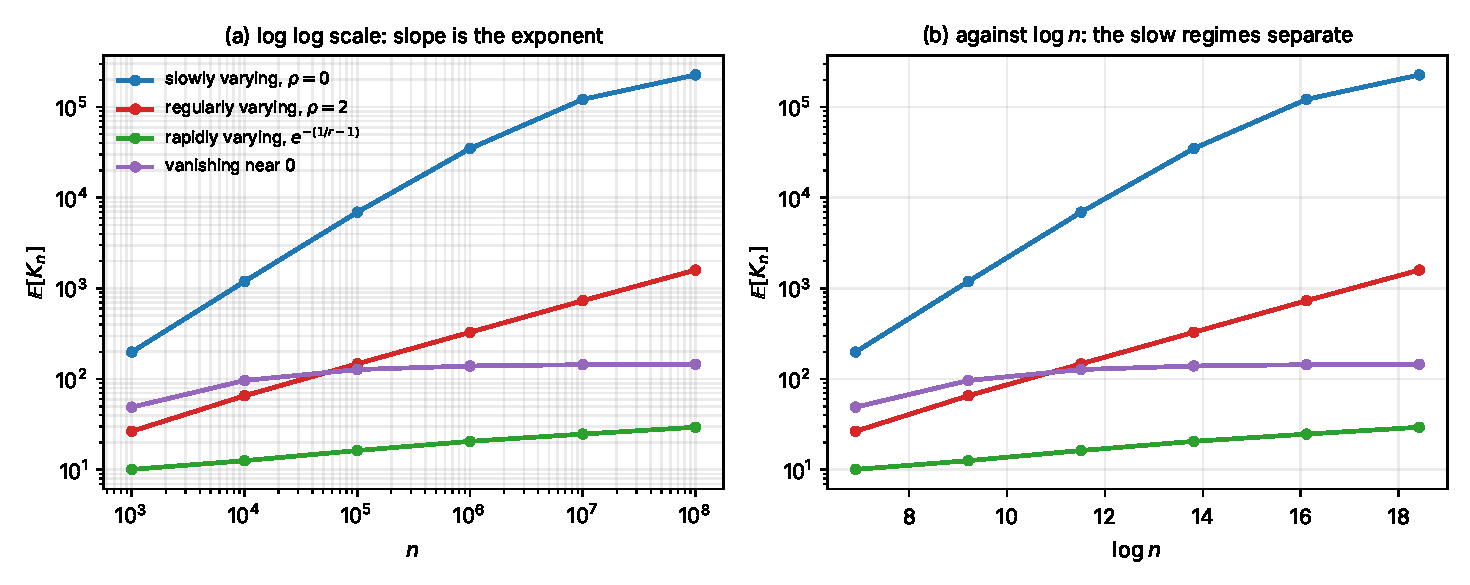
\includegraphics[width=\textwidth]{figures/py_fig-regimes.pdf}
\caption{The four regimes of Theorem~\ref{py:thm:regimes} at $\sigma = \tfrac12$, $\theta = 1$, over
five decades of $n$. Left, on log log axes: the slowly varying and regularly varying weights have
limiting slopes $\sigma_* = 1$ and $\sigma_* = 1/3$. The second is straight. The first bends, its local slope falling from $0.78$ to $0.27$ over
this range, because the $3\times10^{5}$ simulated sticks leave out about a seventh of the probability mass, the rarest types, and with them about forty percent of $\Ex[K_n]$ at $n = 10^{3}$ and ninety eight percent at $n = 10^{8}$; without that loss its slope would be $0.88$ to $0.95$. Right,
the same counts against $\log n$ on a logarithmic vertical scale, which separates the two slow
regimes: the rapidly varying weight keeps climbing, the truncated one has stopped.}
\label{py:fig:regimes}
\end{figure}

\begin{table}[t]
\centering
\caption{Representative weights and their regimes, with the growth of the number of observed types
at $\sigma = \tfrac12$.}
\label{py:tab:examples}
\begin{adjustbox}{max width=\textwidth}
\begin{tabular}{lll}
\toprule
$G(r)$ & regime & $K_n$ at $\sigma = \tfrac12$\\
\midrule
$\{1-\tfrac12\log r\}^{-1}$ & slowly varying, $\rho = 0$ & $n/L(n)$\\
$r^{\rho}$, $\rho > 0$ & regularly varying & $n^{1/(1+\rho)}$\\
$r^{\rho}/(1-\tfrac12\log r)$ & regularly varying, $\ell \not\to c$ & $n^{1/(1+\rho)}L(n)$\\
$\exp\{-(r^{-\tau}-1)\}$ & rapidly varying & $(\log n)^{1/\tau}$\\
$(r-r_0)^{+}/(1-r_0)$ & vanishing near $0$ & bounded\\
\bottomrule
\end{tabular}
\end{adjustbox}
\end{table}

\subsection{What survives, and what needs the power}
\label{py:sec:survives}

The results of Sections~\ref{py:sec:diversity} to \ref{py:sec:joint} fare differently under a general
weight, and the split follows Theorem~\ref{py:thm:rigid} exactly: what depends on the induced
frequencies only through the tail of their counting function survives, and what depends on the
induced subdivision being a residual allocation model does not.

\emph{The spectrum degeneracy survives in full.} Proposition~\ref{py:prop:joint} used only that the
counting function is regularly varying with index $-\sigma_*$, which is
Proposition~\ref{py:prop:index}. So the profile $A_j/K_n \to q_j(\sigma_*)$ of \eqref{py:eq:joint} holds for every weight in regime (ii), Beta or
not, and with it the singleton fraction.

\begin{corollary}
\label{py:cor:anyweight}
For every weight of index $\rho \in (0,\infty)$ in the sense of Proposition~\ref{py:prop:index}, $A_1/K_n \to \sigma_*$ almost surely, and
\[
\hat\sigma \;=\; \frac{\rho\hat\sigma_*}{\rho\hat\sigma_* + 1 - \hat\sigma_*},
\qquad \hat\sigma_* = A_1/K_n,
\]
is consistent for $\sigma$.
\end{corollary}

Figure~\ref{py:fig:index} is the claim in picture form. Three weights of index $\rho = 2$ but quite
different shapes, a pure power, a power times a slowly varying factor, and a power times a
polynomial, all drive $A_1/K_n$ to the same $\sigma_* = 1/3$. At $n = 10^{8}$ they read $0.336$,
$0.312$ and $0.332$, the middle one slowest because its slowly varying factor does not settle. So
correcting a survey drawn with an unknown effort profile does not need the profile. It needs a single
number, the index of $G$ at the far end of the transect, and nothing else about $f$ matters even in
principle. Two collectors with wildly different habits but the same $\rho$ produce statistically
indistinguishable catches at this order.

\begin{figure}[t]
\centering
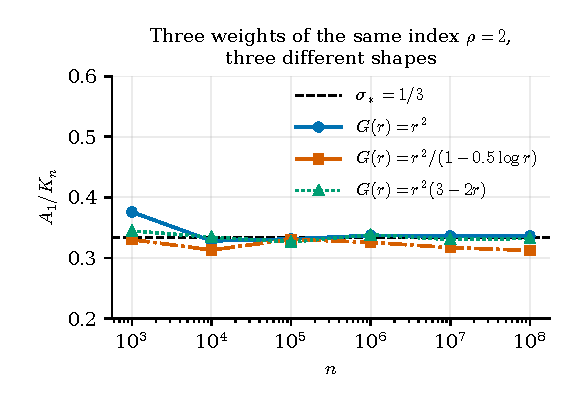
\includegraphics[width=0.7\textwidth]{figures/py_fig-index.pdf}
\caption{Only the index matters. Three weights with $\rho = 2$ and different shapes, at
$\sigma = \tfrac12$, $\theta = 1$: the singleton fraction converges to $\sigma_* = 1/3$ for all
three, most slowly for the weight whose slowly varying factor does not settle.}
\label{py:fig:index}
\end{figure}

\emph{The index can be read off the positions, which breaks the confounding.} In an observational
survey $\rho$ is unknown. But recorded positions $X_i$ are an i.i.d.\ sample from $f$, and $\rho$ is
by definition the lower tail index of $Y = 1-X$, since $\Pr(Y \le y) = G(y) = \ell(y)y^{\rho}$.
Estimating a regular variation index from extreme order statistics is Hill's
problem, with Hill's answer \citep{py:hill1975}.

\begin{corollary}
\label{py:cor:hill}
Let $Y_{(1)} \le \dots \le Y_{(n)}$ be the ordered values of $1-X_i$, and for $m = m_n \to \infty$
with $m/n \to 0$ let
\[
\hat\rho \;=\; \Big\{\frac1m\sum_{i=1}^{m}\log\frac{Y_{(m+1)}}{Y_{(i)}}\Big\}^{-1}.
\]
Then $\hat\rho \to \rho$ in probability, and Corollary~\ref{py:cor:anyweight} with $\hat\rho$ in place
of $\rho$ is consistent for $\sigma$ from the recorded catch alone.
\end{corollary}

The two ingredients use disjoint information: the abundances give $\sigma_*$ and know nothing about
where the specimens were found, the positions give $\rho$ and know nothing about which species they
belonged to. Numerically, with $10^{6}$ positions and the top $10^{5}$ order statistics, Hill
returns $2.003$ for $G(r) = r^{2}$ and $0.49$ for $G(r) = 2r^{1/2}-r$. For
$G(r) = r^{2}/(1-\tfrac12\log r)$ it returns $2.20$, $2.24$, $2.30$ as $m$ runs through
$10^{3}$, $10^{4}$, $10^{5}$: the slowly varying factor biases Hill upward, the well known behaviour
of the estimator under a nonconstant $\ell$. The same factor biased the exponent fit of
Section~\ref{py:sec:index} towards a larger effective $\rho$ as well; both estimators see the local
index $\rho + d\log\ell/d\log r$, so feeding the Hill $\hat\rho$ into the correction partly
compensates for the bias in $\hat\sigma_*$.

The compensation can be explained heuristically, and the explanation gives a rule for choosing $m$. Write
$\rho(r) = d\log G(r)/d\log r = \rho + d\log\ell/d\log r$ for the local index of $G$ at scale $r$.
Both estimators see a local index rather than $\rho$ itself, and the question is at which scale.

\begin{remark}[Scale matching, a heuristic]
\label{py:rem:scale}
The singleton fraction is governed by the induced frequencies of order $1/n$, which sit at tail sum
scale $r_A(n) \asymp n^{-(1-\sigma)/\{\rho(1-\sigma)+\sigma\}}$, so to first order in the slowly
varying factor $(1-\hat\sigma_*)/\hat\sigma_* \approx \rho(r_A)\,\omega$. Hill's estimator with $m$
order statistics is governed by $G$ at scale $r_H = G^{-1}(m/n)$, so $\hat\rho \approx \rho(r_H)$.
The two scales coincide when $m \asymp n\,G(r_A) \asymp n^{\sigma_*} \asymp K_n$. Hence with
$m_n \asymp K_n$ the composed estimator $\hat\omega = \{(1-\hat\sigma_*)/\hat\sigma_*\}/\hat\rho$ is
free of $\ell$ to first order, and the corrected $\hat\sigma$ is less sensitive to the slowly
varying factor than either ingredient. This is a heuristic, not a proved result: the approximations are first order in the variation of $\ell$ with no error term, and the support for the rule is the arithmetic of the scales together with Table~\ref{py:tab:scale}.
\end{remark}

The rule is memorable: take as many extreme positions as there are observed types. It has the right
order of magnitude rather than a sharp optimum, because the local index varies slowly, so any $m$
within a constant factor of $K_n$ sees nearly the same $\rho(r)$.

Table~\ref{py:tab:scale} tests this at $G(r) = r^{2}/(1-\tfrac12\log r)$, $\sigma = \tfrac12$,
$n = 10^{6}$, where $K_n \approx 150$ and the singleton fraction reads $0.320$ against
$\sigma_* = 1/3$. Correcting with the \emph{true} $\rho = 2$ gives $0.485$, the downward bias of the
abundance side passing straight through. Correcting with Hill's $\hat\rho$ instead gives $0.502$ to
$0.511$ for every $m$ from $50$ to $1000$, within about a hundredth of the truth and on the other side of
it, because the upward bias of Hill offsets the downward bias of the singleton fraction. The
compensation is broad rather than sharp, as the remark predicts, and it degrades only when
$m$ is far above $K_n$, where Hill is looking at a scale the abundances never reach.

\begin{table}[t]
\centering
\caption{The corrected estimate of $\sigma = \tfrac12$ under $G(r) = r^{2}/(1-\tfrac12\log r)$ at
$n = 10^{6}$, as a function of the number $m$ of extreme positions used in Hill's estimator; mean
and standard deviation over $12$ independent position samples, the abundance side held fixed at
$A_1/K_n = 0.320$ with $K_n = 151$. Correcting with the true $\rho = 2$ gives $0.485$.}
\label{py:tab:scale}
\begin{adjustbox}{max width=\textwidth}
\begin{tabular}{rrrrrrrrrr}
\toprule
$m$ & $30$ & $50$ & $100$ & $150$ & $300$ & $1000$ & $3000$ & $10^{4}$ & $10^{5}$\\
\midrule
$\hat\sigma$ & $0.507$ & $0.502$ & $0.503$ & $0.508$ & $0.511$ & $0.508$ & $0.510$ & $0.514$ & $0.520$\\
s.d. & $0.038$ & $0.036$ & $0.023$ & $0.019$ & $0.016$ & $0.007$ & $0.006$ & $0.004$ & $0.001$\\
\bottomrule
\end{tabular}
\end{adjustbox}
\end{table}


\emph{The diversity identity survives only up to the slowly varying factor.}
Proposition~\ref{py:prop:power} used $R'_k = \widetilde R_k^{\alpha}$ exactly, and for a general $G$
one has $R'_k = \ell(\widetilde R_k)\widetilde R_k^{\rho}$ instead. The exponent
$\kappa = \rho\sigma_*/\sigma$ survives; the constant does not, and $K_n n^{-\sigma_*}$ need not
converge at all if $\ell$ oscillates. If $G$ has a density $g$ near the origin with $g(r)/r^{\rho-1} \to \rho c$, $c \in (0,\infty)$, then everything goes
through with $\alpha$ replaced by $\rho$ and an extra factor $c^{\sigma_*}$ in \eqref{py:eq:C}. The
clean diversity theory needs the weight to be asymptotically a power, not merely regularly varying.

\section{A worked example: heavy tailed abundance surveys}
\label{py:sec:example}

The one parameter theory is the right model for a community whose species abundance curve is
logarithmic, and the two parameter family is the right model when it is not. Power law abundance
is the rule rather than the exception in microbial surveys, in word frequency data and in network
degree data. It is exactly what $\sigma > 0$ produces: the number of types in a sample of size $n$
grows like $n^{\sigma}$ rather than like $\log n$. The results above say what
a nonuniform sampling effort does to such a survey, and the answer is arithmetically severe.

Suppose the truth is $\sigma = 0.5$, so that types accumulate like $\sqrt{n}$, and the sampling
effort follows $f_\alpha$. Table~\ref{py:tab:worked} reads off the consequences from
\eqref{py:eq:odds}, \eqref{py:eq:power} and \eqref{py:eq:C}. The column $\sigma_*$ is what an analyst would estimate from the growth of the type count. The
type count ratio is the factor by which that count at $n = 10^{6}$ differs from what uniform
sampling would have produced, namely $n^{\sigma_*-\sigma}$ times the constant of \eqref{py:eq:C}, for a community whose diversity is $S = 1$; in general the factor $S^{\kappa-1}$ multiplies it, and the ratio of mean counts at $\theta = 1$ is $44.0$, $8.31$, $1$, $0.118$ and $0.021$. And
$\kappa$ is the power to which the whole diversity distribution is raised.

\begin{table}[t]
\centering
\caption{Consequences of an effort profile $f_\alpha$ for a community with true discount parameter
$\sigma = 0.5$. The type count ratio is at $n = 10^{6}$ and combines the change of exponent with
the constant \eqref{py:eq:C}.}
\label{py:tab:worked}
\begin{adjustbox}{max width=\textwidth}
\begin{tabular}{rrrrr}
\toprule
$\alpha$ & effort & $\sigma_*$ & $\kappa$ & type count ratio at $n=10^{6}$\\
\midrule
$0.25$ & strongly persistent & $0.800$ & $0.400$ & $73.3$\\
$0.5$  & persistent          & $0.667$ & $0.667$ & $11.1$\\
$1$    & uniform             & $0.500$ & $1.000$ & $1.000$\\
$2$    & fading              & $0.333$ & $1.333$ & $0.086$\\
$4$    & strongly fading     & $0.200$ & $1.600$ & $0.012$\\
\bottomrule
\end{tabular}
\end{adjustbox}
\end{table}

Three things follow. First, the effect is a change of \emph{exponent}, so it compounds with
sample size: a fading collector with $\alpha = 2$ recovers about nine percent of the types a
uniform sample would have found at $n = 10^{6}$, and under three percent at $n = 10^{9}$ (both figures are for $S = 1$; the ratios of mean counts at $\theta = 1$ are twelve percent, as in Example~\ref{py:ex:odds}, and under four percent).
No amount of sampling repairs it, because the deficit grows. This is qualitatively worse than the
one parameter case, where an effort profile changes the constant multiplying $\log n$ and the
relative deficit is fixed.

Second, the direction is not obvious in advance. A persistent collector, one who works harder at
the far end of the transect where the rare types live, inflates the apparent diversity, and at
$\alpha = 0.25$ he reports seventy times too many types when $S = 1$; at $\theta = 1$ the ratio of mean counts is forty four. Ascertainment is not simply loss.

Third, and most useful in practice, the correction \eqref{py:eq:correct} is exact and needs only
$\alpha$. If the effort profile is part of the design, as in a stratified or adaptive survey, then
$\alpha$ is known and the bias is removable in full. If it is not, then $\sigma$ and $\alpha$ enter the type count only through $\sigma_*$ and are not
separately identifiable from it. The confounding that Bayarri and DeGroot describe for weighted
distributions in general appears here in its sharpest form, as a single ratio.

\section{What remains}
\label{py:sec:remains}

Three problems are left, the last of them a matter of refinement.

\emph{The random envelope in the bias calculation.} Proposition~\ref{py:prop:rate} gives the bias
of the singleton fraction under a deterministic envelope, and finds it negligible. The sandwich
argument of Lemma~\ref{py:lem:MS} controls the leading order of the random case but not the
$O(1/K_n)$ term, where the fluctuation of the Gamma factors about their mean contributes at the same
order as the $-\tfrac12$ from the zeta function. Carrying the Mellin calculation through with the
Gamma noise included, and doing the same for $1-2A_2/A_1$, is the natural next step. Neither
question is the simulation difficulty of Section~\ref{py:sec:truncation}: a real survey has no
truncated stick, so \eqref{py:eq:trunc} constrains our numerics and not the estimator.

\emph{Two parameter weights.} Theorem~\ref{py:thm:rigid} closes the question, for densities that charge every interval and in the stick breaking sense, for weights acting as
$G(R_k)$ on the tail sums. It says nothing about ascertainment schemes that are not of this form,
for instance those depending on the atom index as well as its position. Whether some such scheme
preserves Ewens Pitman is open.

\emph{Second order scale matching.} Remark~\ref{py:rem:scale} cancels the slowly varying factor
to first order by matching the scales at which the two estimators read the local index. The
residual, which Table~\ref{py:tab:scale} shows to be about a hundredth here, comes from the variation
of $\rho(r)$ across the two windows and from the fact that the abundance side averages over a range
of scales while Hill averages over another. Identifying the constant in $m \asymp K_n$ that
minimises it, and the second order term itself, would turn a rule of thumb into a procedure.

\section{Summary}
\label{py:sec:summary}

\begin{table}[t]
\centering
\caption{What the ascertainment calculus does to the two families.}
\label{py:tab:summary}
\begin{tabularx}{\textwidth}{>{\raggedright\arraybackslash}p{1.35in}>{\raggedright\arraybackslash}X>{\raggedright\arraybackslash}X}
\toprule
& one parameter, $\sigma = 0$ & two parameter, $\sigma > 0$ \\
\midrule
the reduction & holds & holds, unchanged \\
genealogical construction & defining events, $\theta/\alpha$ & feedback or multiple mergers \\
layout matters for exactness & yes & yes \\
layout matters for leading order & no (Prop~\ref{py:prop:ranked0}) & no (Prop~\ref{py:prop:layout}) \\
direction of layout & \multicolumn{2}{l}{absorbed into $G$ (Lemma~\ref{py:lem:reflect})} \\
family preserved & yes, $\theta \mapsto \theta/\alpha$ & no, by no weight charging every interval
  (Thm~\ref{py:thm:rigid}) \\
image of the weighting & $\GEM(\theta/\alpha)$ & explicit RAM, \eqref{py:eq:image} \\
growth of $K_n$ & $(\theta/\alpha)\log n$ & $n^{\sigma_*+o(1)}$ \\
parameter rescaled & $\theta \mapsto \theta/\alpha$ &
  $(1-\sigma)/\sigma \mapsto \alpha(1-\sigma)/\sigma$ \\
role of the other parameter & $\cdot$ & $\theta$ absent from $\sigma_*$ and from $C$ \\
limit law of the diversity & degenerate & $C\,S^{\kappa}$, $C$ by \eqref{py:eq:C} \\
limit of $(A_j)$ & independent Poisson$(\vartheta/j)$ & $q_j(\sigma_*)S_*$, degenerate \\
coincidence probability & $\to e^{-\gamma\vartheta}/\Gamma(1+\vartheta)$ & $\to 0$, any weight with $\sigma_* > 0$ \\
correction for a biased sample & $\theta = \alpha\vartheta$ & \eqref{py:eq:correct} \\
estimator of the parameter & $K_n/\log n$ & $A_1/K_n$, or $1-2A_2/A_1$ \\
arbitrary weight, index $\rho$ & $K_n \sim (\theta/\rho)\log n$ &
  $\alpha \mapsto \rho$ throughout; four regimes \\
\bottomrule
\end{tabularx}
\end{table}

In one sentence: the reduction is universal in the law of the subdivision and in the direction it
is laid down; exactness is the Ewens case and no other weight that charges every interval rescues it; the first order rescaling
generalises with the odds $(1-\sigma)/\sigma$ in place of $\theta$; the limiting diversity is the
unweighted one raised to the power $\kappa$, by a map free of $\theta$; and the coincidence theory
does not generalise at all.

\section{Exercises}
\label{py:sec:exercises}

\begin{enumerate}[label=\arabic*., leftmargin=*]
\item Verify the $n = 4$ column for $(\sigma,\theta) = (\tfrac14,2)$ in Table~\ref{py:tab:eppf}
directly from \eqref{py:eq:eppf}, and check that the column sums to one.
\emph{Hint.} The denominator is $(3)_3 = 60$; the multiplicities are $1, 4, 3, 6, 1$.

\item Show that under $\PD(\sigma,\theta)$ the probability that $n$ uniformly sampled points are all
distinct is $\prod_{i=1}^{n-1}(\theta+i\sigma)/(\theta+1)_{n-1}$, and that it tends to zero for
every $\sigma < 1$.
\emph{Hint.} Take all $n_j = 1$ in \eqref{py:eq:eppf}; for the limit note that the
$i$th factor $(\theta+i\sigma)/(\theta+i)$ tends to $\sigma < 1$.

\item Let $1-B \sim \Beta(\theta,1)$. Show that $(1-B)^{\alpha} \sim \Beta(\theta/\alpha,1)$, and
deduce that the weighted image of a size biased $\GEM(\theta)$ subdivision under
$f_\alpha(x) = \alpha(1-x)^{\alpha-1}$ is $\GEM(\theta/\alpha)$.
\emph{Hint.} Compute $\Pr\{(1-B)^{\alpha} \le v\}$ and use Lemma~\ref{py:lem:pit} with
$G(r) = r^{\alpha}$.

\item Under $\ESF(\theta)$ the homozygosity is $1/(1+\theta)$. Show that a collector who samples a
size biased $\GEM(\theta)$ subdivision with $f_\alpha$ observes homozygosity $\alpha/(\alpha+\theta)$,
and find the $\alpha$ that doubles it when $\theta = 3$.
\emph{Hint.} Use Exercise 3; the answer is $\alpha = 3$.

\item Prove the composition law $T_\alpha\circ T_{\alpha'} = T_{\alpha\alpha'}$ of
Proposition~\ref{py:prop:group} directly from the formula
$T_\alpha(\sigma) = \sigma/\{\alpha(1-\sigma)+\sigma\}$, without the odds coordinate.
\emph{Hint.} Compute $1/T_\alpha(\sigma) - 1$.

\item Show that $\kappa = \alpha\sigma_*/\sigma$ satisfies the composition rule
\eqref{py:eq:kappacomp}.
\emph{Hint.} Write $\kappa(\sigma,\alpha) = \alpha/\{\alpha(1-\sigma)+\sigma\}$ and use
$1-T_{\alpha'}(\sigma) = \alpha'(1-\sigma)/\{\alpha'(1-\sigma)+\sigma\}$.

\item Show that the Sibuya probabilities $q_j(\sigma)$ of \eqref{py:eq:joint} satisfy
$q_{j+1}/q_j = (j-\sigma)/(j+1)$, and deduce that $A_2/A_1 \to (1-\sigma_*)/2$ and
$A_3/A_2 \to (2-\sigma_*)/3$. Propose a third estimator of $\sigma_*$ from $A_3/A_2$ and compute it
for the Shakespeare data of Example~\ref{py:ex:shakespeare}.
\emph{Hint.} $\Gamma(j+1-\sigma) = (j-\sigma)\Gamma(j-\sigma)$; the estimate is
$2 - 3(2292)/4343 = 0.417$.

\item A survey reports $K_n = 640$ types of which $A_1 = 192$ are singletons, collected with a
design known to have $\alpha = 3$. Estimate $\sigma_*$ and $\sigma$, and give an approximate
standard error for each.
\emph{Hint.} $\hat\sigma_* = 0.30$ and $\hat\sigma = 0.5625$; use
$\{\hat\sigma_*(1-\hat\sigma_*)/K_n\}^{1/2}$ and the delta method factor
$\sigma(1-\sigma)/\{\sigma_*(1-\sigma_*)\}$.

\item Let $f(x) = 6x(1-x)$ and lay the intervals from the left. Find the index $\rho$ of $G$ at the
origin, and hence $\sigma_*$ when $\sigma = \tfrac12$. Repeat for $f(x) = 2x$.
\emph{Hint.} Proposition~\ref{py:prop:contact}: $f(x) \sim 6(1-x)$ at $x = 1$ gives $\rho = 2$ and
$\sigma_* = 1/3$; $f(x) = 2x$ tends to $2$ at $x = 1$, so $\rho = 1$ and $\sigma_* = \tfrac12$.

\item The defining event construction of Proposition~\ref{py:prop:nocoal} gives
$K_3 = 1 + \xi_2 + \xi_3$ with independent $\xi_j \sim \mathrm{Bernoulli}(p_j)$. Show that no choice
of $p_2, p_3 \in [0,1]$ reproduces the law of $K_3$ under $\PD(\tfrac12,1)$, so the obstruction is
visible already at $n = 3$, before any variance comparison can detect it.
\emph{Hint.} From Table~\ref{py:tab:eppf}, $\Pr(K_3 = 1) = 1/8$ and $\Pr(K_3 = 3) = 1/2$; these force
$p_2+p_3 = 11/8$ and $p_2p_3 = 1/2$, and the quadratic with these roots has negative discriminant.

\item (Computation.) Implement the moment recursion of Example~\ref{py:ex:n4} and reproduce the
$\alpha = 2$ column of Table~\ref{py:tab:n4}. Then vary $\alpha$ over $(0,5)$ and plot the ratio
for the type $2{+}2$; confirm that it equals one at $\alpha = 1$.
\emph{Hint.} Run the recursion backwards from a truncation index of $10^{5}$; all moments are Beta
function ratios, best computed through log gamma functions.

\item (Computation.) Simulate a ranked $\PD(\tfrac12,1)$ subdivision, sample it with $f_2$, and
compare $A_1/K_n$ at $n = 10^{6}$ with the value $1/3$ given by Proposition~\ref{py:prop:layout}
and Corollary~\ref{py:cor:singleton}.
\emph{Hint.} Generate size biased sticks, sort them, and use \eqref{py:eq:trunc} to choose the
number of sticks; Rao Blackwellise the counts as in Table~\ref{py:tab:joint}.
\end{enumerate}

\begin{thebibliography}{}

\bibitem[Arratia, Barbour and Tavar\'e(2003)]{py:arratia2003}
Arratia, R., Barbour, A. D. and Tavar\'e, S. (2003). \emph{Logarithmic Combinatorial Structures: A
Probabilistic Approach}. European Mathematical Society, Z\"urich.

\bibitem[Berestycki, Berestycki and Schweinsberg(2007)]{py:berestycki2007}
Berestycki, J., Berestycki, N. and Schweinsberg, J. (2007). Beta coalescents and continuous stable
random trees. \emph{The Annals of Probability} 35, 1835 to 1887.

\bibitem[Birkner et~al.(2005)]{py:birkner2005}
Birkner, M., Blath, J., Capaldo, M., Etheridge, A., M\"ohle, M., Schweinsberg, J. and
Wakolbinger, A. (2005). Alpha stable branching and beta coalescents. \emph{Electronic Journal of
Probability} 10, 303 to 325.

\bibitem[Efron and Thisted(1976)]{py:efron1976}
Efron, B. and Thisted, R. (1976). Estimating the number of unseen species: how many words did
Shakespeare know? \emph{Biometrika} 63, 435 to 447.

\bibitem[Ewens(1972)]{py:ewens1972}
Ewens, W. J. (1972). The sampling theory of selectively neutral alleles. \emph{Theoretical
Population Biology} 3, 87 to 112.

\bibitem[Fisher(1934)]{py:fisher1934}
Fisher, R. A. (1934). The effect of methods of ascertainment upon the estimation of frequencies.
\emph{Annals of Eugenics} 6, 13 to 25.

\bibitem[Fisher, Corbet and Williams(1943)]{py:fisher1943}
Fisher, R. A., Corbet, A. S. and Williams, C. B. (1943). The relation between the number of
species and the number of individuals in a random sample of an animal population.
\emph{Journal of Animal Ecology} 12, 42 to 58.

\bibitem[Hill(1975)]{py:hill1975}
Hill, B. M. (1975). A simple general approach to inference about the tail of a distribution.
\emph{The Annals of Statistics} 3, 1163 to 1174.

\bibitem[Karlin(1967)]{py:karlin1967}
Karlin, S. (1967). Central limit theorems for certain infinite urn schemes. \emph{Journal of
Mathematics and Mechanics} 17, 373 to 401.

\bibitem[Kingman(1978)]{py:kingman1978}
Kingman, J. F. C. (1978). The representation of partition structures. \emph{Journal of the London
Mathematical Society} 18, 374 to 380.

\bibitem[M\"ohle(2010)]{py:mohle2010}
M\"ohle, M. (2010). Asymptotic results for coalescent processes without proper frequencies and
applications to the two parameter Poisson Dirichlet coalescent. \emph{Stochastic Processes and
their Applications} 120, 2159 to 2173.

\bibitem[Patil and Rao(1978)]{py:patil1978}
Patil, G. P. and Rao, C. R. (1978). Weighted distributions and size biased sampling with
applications to wildlife populations and human families. \emph{Biometrics} 34, 179 to 189.

\bibitem[Pitman(1995)]{py:pitman1995}
Pitman, J. (1995). Exchangeable and partially exchangeable random partitions. \emph{Probability
Theory and Related Fields} 102, 145 to 158.

\bibitem[Pitman(1999)]{py:pitman1999}
Pitman, J. (1999). Coalescents with multiple collisions. \emph{The Annals of Probability} 27,
1870 to 1902.

\bibitem[Pitman(2006)]{py:pitman2006}
Pitman, J. (2006). \emph{Combinatorial Stochastic Processes}. Lecture Notes in Mathematics 1875,
Springer, Berlin.

\bibitem[Pitman and Yor(1997)]{py:pitmanyor1997}
Pitman, J. and Yor, M. (1997). The two parameter Poisson Dirichlet distribution derived from a
stable subordinator. \emph{The Annals of Probability} 25, 855 to 900.

\bibitem[Rao(1965)]{py:rao1965}
Rao, C. R. (1965). On discrete distributions arising out of methods of ascertainment.
\emph{Sankhy\=a A} 27, 311 to 324.

\bibitem[Sagitov(1999)]{py:sagitov1999}
Sagitov, S. (1999). The general coalescent with asynchronous mergers of ancestral lines.
\emph{Journal of Applied Probability} 36, 1116 to 1125.

\bibitem[Sethuraman(1994)]{py:sethuraman1994}
Sethuraman, J. (1994). A constructive definition of Dirichlet priors. \emph{Statistica Sinica} 4,
639 to 650.

\end{thebibliography}
